% !TEX program = xelatex
\documentclass[UTF8]{ctexrep}
\usepackage{xeCJK}
\setCJKmainfont[BoldFont=HiraginoSansGB-W3, ItalicFont=AdobeKaitiStd-Regular]{FZXSSJW--GB1-0}
\setCJKsansfont{HiraginoSansGB-W6}
\setCJKmonofont{FZLTXHK--GBK1-0}
\CTEXsetup[format+={\raggedright}]{section}

\usepackage{fontspec}
\setmainfont{TimesNewRomanPSMT}
\setsansfont{Verdana}
\setmonofont{Menlo-Regular}

\newfontfamily{\FAB}{Font Awesome 5 Brands Regular}
\setCJKfamilyfont{FZFS}{FZFENSTXJW--GB1-0}
\newfontfamily{\FAFR}{Font Awesome 5 Free Regular}
\def\faGithub{{\FAB \symbol{"F09B}}} % Github
\def\faEmail{{\FAFR \symbol{"F0E0}}} % E-Mail

\usepackage{float}

\usepackage{geometry}
\geometry{a4paper,left=3cm,right=3cm,top=2.5cm,bottom=2.5cm}

\usepackage{fancyhdr}
\pagestyle{fancy}
\fancyhf{}
\chead{\itshape 现代密码学简介}
\rhead{\thepage}
\renewcommand\headrulewidth{0.6pt}

\makeatletter
\renewcommand\chapter{\if@openright\cleardoublepage\else\clearpage\fi
    \thispagestyle{fancy}% original style: plain
    \global\@topnum\z@
    \@afterindentfalse
    \secdef\@chapter\@schapter%
}
\makeatother

\renewcommand{\labelitemii}{$\circ$}

\usepackage{amsmath}
\usepackage{esvect}
\usepackage{bm}
\usepackage{upgreek}
\def \paral {/\!/}
\usepackage{mathtools}
\usepackage{amssymb}
\usepackage{extarrows}
\usepackage{mathrsfs}
\usepackage[amssymb]{SIunits}
\renewcommand{\epsilon}{\varepsilon}
\newcommand{\ext}{\displaystyle}
\newcommand{\arsinh}{\mathrm{arsinh}\,}
\newcommand{\arcosh}{\mathrm{arcosh}\,}
\newcommand{\artanh}{\mathrm{artanh}\,}
\newcommand{\dif}{\mathop{}\!{}\mathrm{d}}
\newcommand{\ic}{\mathrm{i}}
\newcommand{\Tr}{\mathrm{T}}
\newcommand{\ke}{\mathrm{k}}
\newcommand{\p}{\mathrm{p}}
\newcommand{\Z}{\mathbb{Z}}

\def\mathbm#1{{\bm #1}}
\def\vec#1{\vv{\bm #1}}
\def\xvec#1#2{\vv{{\bm #1}_{#2}}}
\def\yvec#1#2{\vv{{\bm #1}^{#2}}}
\def\abs#1{\left| #1 \right|}
\def\pth#1{\left( {#1}\right)}
\def\brack#1{\left[ {#1}\right]}
\def\brace#1{\left\{ {#1} \right\}}
\def\E#1#2{{\mathrm{E}_{#1}\left({#2}\right)}}
\def\D#1#2{{\mathrm{D}_{#1}\left({#2}\right)}}
\def\GF{\mathrm{GF}}
\def\ID{\mathrm{ID}}
\renewcommand{\rem}{{\bfseries Remark}}

\usepackage{amsthm}

\newtheorem{Definition}{\hspace{2em}定义}[chapter]
\newtheorem{theorem}{\hspace{2em}定理}[chapter]

\usepackage[framemethod=tikz]{mdframed}
\newenvironment{prove}{\begin{mdframed}[backgroundcolor=gray!10,roundcorner=8pt]}{\end{mdframed}}

\title{现代密码学简介}
\author{张曙}
\date{\today}

\usepackage{titlesec}%manage the title
\titleclass{\subsubsubsection}{straight}[\subsection]

\newcounter{subsubsubsection}[subsubsection]
\renewcommand\thesubsubsubsection{\thesubsubsection.\arabic{subsubsubsection}}
\renewcommand\theparagraph{\thesubsubsubsection.\arabic{paragraph}} % optional; useful if paragraphs are to be numbered

\titleformat{\subsubsubsection}
  {\normalfont\normalsize\bfseries}{\thesubsubsubsection}{1em}{}
\titlespacing*{\subsubsubsection}
{0pt}{3.25ex plus 1ex minus .2ex}{1.5ex plus .2ex}

\makeatletter
\renewcommand\paragraph{\@startsection{paragraph}{5}{\z@}%
  {3.25ex \@plus1ex \@minus.2ex}%
  {-1em}%
  {\normalfont\normalsize\bfseries}}
\renewcommand\subparagraph{\@startsection{subparagraph}{6}{\parindent}%
  {3.25ex \@plus1ex \@minus .2ex}%
  {-1em}%
  {\normalfont\normalsize\bfseries}}
\def\toclevel@subsubsubsection{4}
\def\toclevel@paragraph{5}
\def\toclevel@paragraph{6}
\def\l@subsubsubsection{\@dottedtocline{4}{7em}{4em}}
\def\l@paragraph{\@dottedtocline{5}{10em}{5em}}
\def\l@subparagraph{\@dottedtocline{6}{14em}{6em}}
\makeatother

\usepackage[absolute]{textpos}

\usepackage[unicode]{hyperref}
\hypersetup{pdfauthor={张曙},
pdftitle={现代密码学简介},
hidelinks
}
\begin{document}
\begin{titlepage}
\vspace*{9em}{\centering\Huge\CJKfamily{FZFS} 现代密码学简介\par}
\vspace{5em}{\centering\Large \textbf{张曙}\par}
\vspace{3em}{\centering\faGithub\quad\texttt{\href{https://github.com/Evian-Zhang}{https://github.com/Evian-Zhang}}\par\centering\faEmail\quad\texttt{\href{mailto:evianzhang1999@gmail.com}{evianzhang1999@gmail.com}}\par}
\begin{textblock}{10}[0,0](3,14)
在GitHub上查看本项目:\faGithub\quad\texttt{\href{https://github.com/Evian-Zhang/Introduction-to-modern-cryptography}{Evian-Zhang/Introduction-to-modern-cryptography}}
\end{textblock}
\end{titlepage}
\tableofcontents
\thispagestyle{fancy}
\input{chapters/chapter_1/绪论}
\input{chapters/chapter_2/流密码与伪随机数发生器}
% !TEX root = 现代密码学简介.tex
\chapter{分组密码}
\section{设计密码系统的方法}
我们之前提到如凯撒密码、多表代换密码等经典密码的时候,讲到了破解这些密码的一种方法,就是利用英文中每个字母出现的频率不同。一次一密的方法可以抵御这种破解,原因是对于明文中的每个字符,其移位都是随机的,因此在密文中完全没有明文中字母出现的频率的信息。但是,一次一密的成本又太高,我们有没有什么办法,能尽可能地掩盖在密文中出现的字母频率的信息,来抵御这种频率攻击呢?香农给出了一种解决方法。
\subsection{扩散与混淆}
所谓扩散,指的是如果我们改变明文中的一个字符,加密得到的密文中的多个字符也会得到改变;如果我们改变密文中的一个字符,解密得到的明文中的多个字符也同样会得到改变。因此,明文中一个字符的信息被“扩散”到密文中的多个字符。因此,实现扩散的方法,就可以是用明文中的多个字符去生成密文中的一个字符。\par
扩散是将明文和密文之间的关系变得复杂使我们很难获得密钥,而混淆则是将密钥和密文之间的关系变得复杂。例如,密钥中的一个字符的改变会导致密文中多个字符的改变。因此,即使攻击者通过密文,知道了一些关于明文的统计信息,也很难获得密钥。\par
我们可以发现,凯撒密码的加密方式并没有实现扩散和混淆,因此,它可以被频率攻击轻易破解。
\subsection{置换与代换}
为了实现扩散,常用的方法是置换。也就是说,把输入的一部分与另一部分进行交换,然后输出。置换中最常用的结构为P盒。其接受$m$位二进制输入,$m$位二进制输出。其输出是把输入的比特按一定规则打乱顺序后输出。\par
为了实现混淆,常用的方法是代换。而代换中最常用的结构为S盒。其接受$m$位二进制输入,$n$位二进制输出。因此,其输入共有$2^m$中,输出共有$2^n$种。我们可以把S盒理解成一种查找表。对于$2^m$个输入中的每一种输入,我们可以在这个表中查找到一个$n$位的输出,而且S盒需要保证不同的输入对应的输出也不同。从编程上,我们也可以将此理解成一个长度为$2^m$的数组,它的每个元素为$n$比特的数字。因此,其所占的空间为$n2^m$.
\section{分组密码的定义}
事实上,在非对称密码发展之前,大多数著名的密码体系,其核心都是扩散与混淆。但是,在我们上述谈到扩散与混淆的时候,有一个值得注意的地方:实现扩散与混淆的器件,即P盒与S盒,其接受的都是固定长度的输入。这与我们之前谈到的流密码不同,流密码的输入可以是任意长度的。因此,为了更好地实现扩散与混淆,我们引入了分组密码。\par
分组密码就是一个较好地实现扩散与混淆的密码系统。它的核心思想是分组。首先,将明文分成若干个等长的组,然后对每个组利用密钥依次进行加密,生成等长的密文组。\par
对于分组密码,我们要研究的有:每组内如何根据输入和密钥进行加密,以及各组之间的关系。最简单的方法是各组的输入是之前分好的明文的各个分组,密钥是相同的密钥。但是,也可以使用相对复杂的方法,使加密变得更加复杂(参见“分组密码的运行模式”一节)。\par
由于密文是明文按组生成的,因此,分组密码具有扩散性;而通过采用特别设定的S盒,也可以实现混淆性。\par
这里我们要注意的是,密码学中研究的分组密码,并不仅仅是将明文分组的加密方式。我们之前提到的同步密码,实际上也可以看作是将明文分组进行加密,每个组的长度为其伪随机密钥流的周期。但是,同步流密码依然是逐比特加密,因此,失去了扩散性。所以,只有这个组的每个比特都参与到了密文的生成中的加密方法,才是我们这一章研究的重点。\par
此外,在讨论为分组密码的运行模式,即各组之间的联系之后,我们接下来讨论的DES, IDEA, AES等都是每组内的加密方法。由于分好了组,所以这些密码体制有一个特点,即明文或者密文是固定长度的。
\section{分组密码的设计方法}
之前讲到,对于分组密码,我们要研究的有:每组内如何根据输入和密钥进行加密,以及各组的输入和密钥是什么。本节讨论的是每组内的加密方法。也就是说,在本节内,我们提到的“输入”、“明文”等,都是指被分好组以后的每个组的输入、明文。\par
常见的分组密码有两种核心设计方法:费斯妥密码与SP网络。它们都有一个相同的特点:需要将同一个步骤重复多轮。而在加密过程中,任何核心步骤都是同时需要明文和密钥的信息的。因此,为了保证可靠性,每一轮步骤的输入和密钥都是不一样的。步骤的输入可以根据上一轮的输出来改变,而密钥怎么办呢?这时,就需要\textbf{子密钥}。所谓子密钥,就是根据密钥,生成的不同序列。比如说,某种方法需要16轮步骤,那么,我们就应设计一种算法,使密钥能生成16个子密钥。
\subsection{费斯妥密码}
费斯妥密码每一轮的步骤,接受上一轮的输出$O_{i-1}$为本轮的输入$I_i$, 同时接受子密钥$K_i$, 输出本轮输出$O_i$.\par
首先,将输入的二进制串$O_{i-1}$分成左右两个相等长度的子串$L_{i-1}$和$R_{i-1}$, 然后计算
\begin{gather}
    L_{i}=R_{i-1}\\
    R_{i}=L_{i-1}\oplus F\pth{R_{i-1}, K_i}
\end{gather}

最后输出是把$L_i$和$R_i$拼起来成$O_i$.\par
其中$F\pth{R_{i-1}, K_i}$称为轮函数,是不同具体的加密算法的核心。\par
而由于等式$a\oplus b\oplus b=a$, 因此,其解密过程与加密过程完全相同,只不过需要把子密钥倒着顺序使用。\par
可以用下图形象地理解费斯妥密码(图源wiki):
\begin{figure}[H]
    \centering
    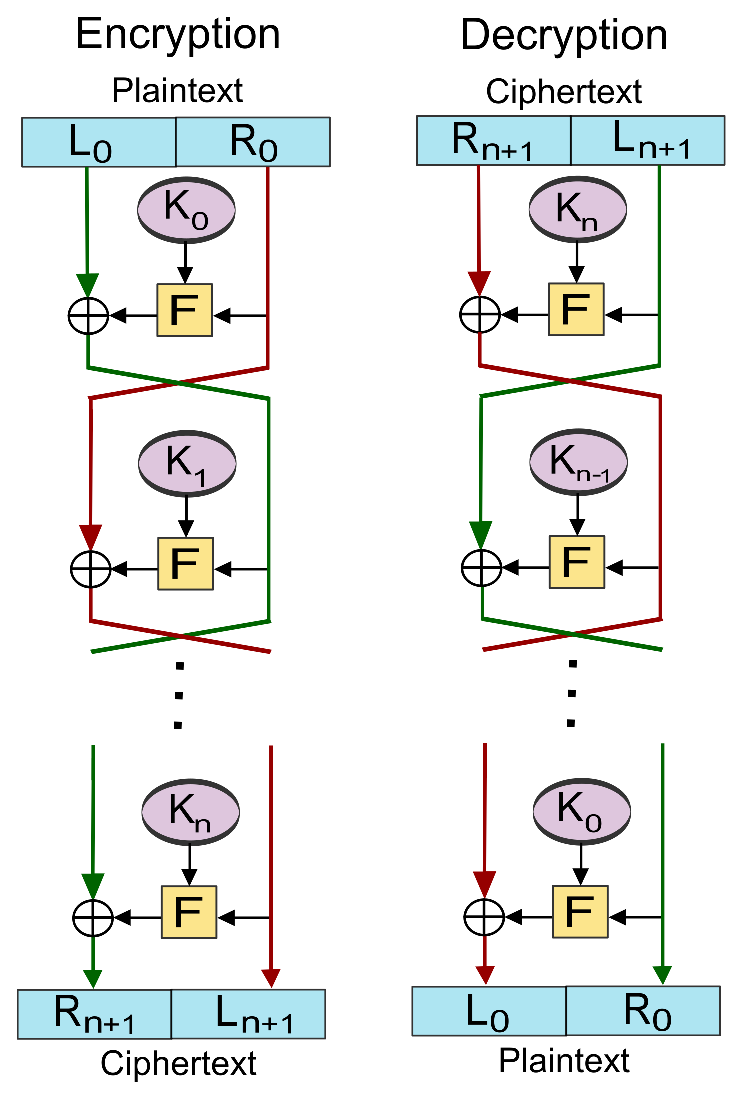
\includegraphics[scale=0.8]{chapters/chapter_3/Feistel.eps}
\end{figure}

值得注意到的一点是,在最后一次输出的时候,不再进行交换,也就是说,输出的并不是$\pth{L_{n+1}, R_{n+1}}$, 而是$\pth{R_{n+1}, L_{n+1}}$.
\subsection{SP网络}
SP网络每轮接受到输入之后,首先,将输入与该轮的子密钥进行异或,然后是对输入再次分组(也就是对分过组的明文的每组内容再次进行分组),接着将每个组通过不同的S盒进行代换,代换后的结果再拼成一个新的串,经过一个P盒的置换进行输出。\par
可以通过下图形象地理解SP网络(图源wiki):
\begin{figure}[H]
    \centering
    \includegraphics[scale=0.5]{chapters/chapter_3/SPN.png}
\end{figure}
\section{分组密码的运行模式}
上一节讨论了在对明文分好组后,每组内常见的加密方式。本节讨论的,则是组与组之间输入和输出的关系。在这里,假设将明文$M$分成了$m_1, m_2, \ldots, m_n$共$n$个等长的组,在每组内,加密算法为$\E{k}{m}$, 解密算法为$\D{k}{c}$.
\subsection{电码本模式(ECB)}
对于每组,其加密的输入为明文分好的组$m_i$, 密钥为同一个密钥串$k$. 也就是说,
\begin{equation}
c_i=\E{k}{m_i}
\end{equation}

其加密过程如图所示(图源wiki):
\begin{figure}[H]
\centering
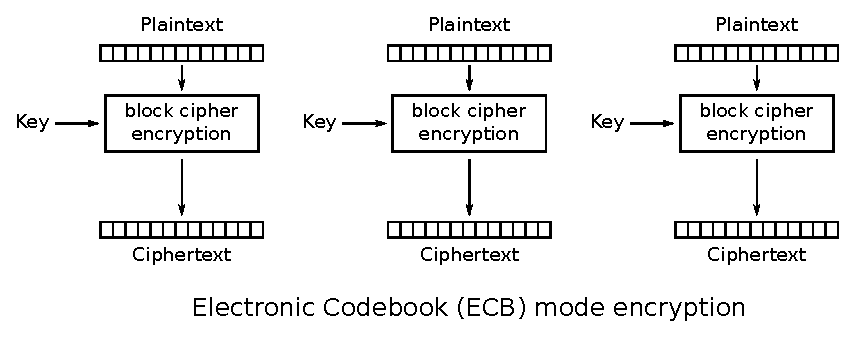
\includegraphics[scale=1]{chapters/chapter_3/ECB.eps}
\end{figure}

ECB模式极不安全。比如说,我想用ECB模式的AES密码体系加密东南大学的校徽:
\begin{figure}[H]
\centering
\includegraphics[width=10em]{chapters/chapter_3/ECB_origin.jpg}
\end{figure}

结果为
\begin{figure}[H]
\centering
\includegraphics[width=10em]{chapters/chapter_3/ECB_result.jpg}
\end{figure}
\subsection{密码分组链接模式(CBC)}
对于每组,其加密的输入为当前明文组与前一密文组的异或。也就是说,
\begin{equation}
c_i=\E{k}{m_i\oplus c_{i-1}}=\E{k}{m_i\oplus \E{k}{m_{i-1}}}
\end{equation}

对于第一组明文组,由于没有$m_0$, 因此,需要一个初始的二进制串,常记作$IV$, 来与$m_1$异或。\par
其加密过程如图所示(图源wiki):
\begin{figure}[H]
\centering
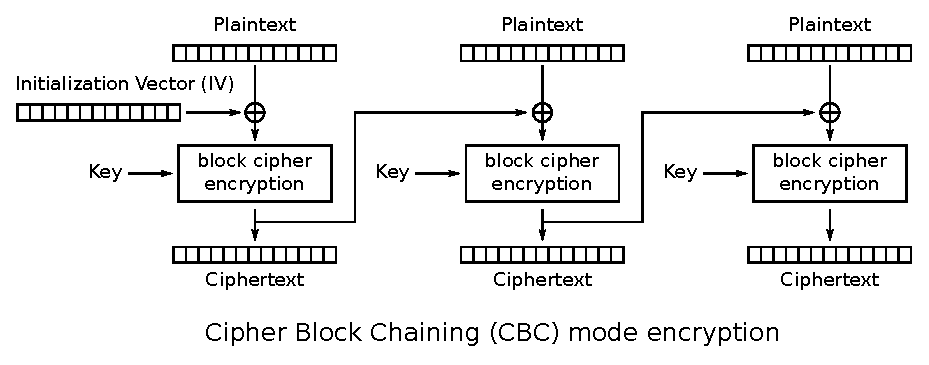
\includegraphics[scale=1]{chapters/chapter_3/CBC.eps}
\end{figure}
\subsection{密码反馈模式(CFB)}
CFB模式需要一个移位寄存器。同时,CFB模式也提供了一个可选的参数$j$, 通常取$j=8$. 其过程如下:\par
对于每组,首先需要进一步分组,使每组的长度为$j$个比特。然后对于每个新分好的组,先将移位寄存器左移$j$个比特,然后将上一组输出的$j$个比特输入到移位寄存器的右边。然后将移位寄存器内存储的二进制串用密钥$k$进行加密,其输出取前$j$个比特与本组的$j$个比特的输入进行异或输出。\par
与CBC类似,处理第一组时移位寄存器内的值也需要一组初始的二进制串$IV$.\par
因此,如果记$H_j(m)$代表取$m$的左边$j$位,$P_i$表示将每组进一步分为的$j$比特的分组,则CFB模式的加密过程可用公式描述为:
\begin{equation}
c_i=H_j\pth{\E{k}{S_{i-1}}}\oplus P_i
\end{equation}
其中$S_i$为移位寄存器的值。移位寄存器的工作方式为
\begin{equation}
S_i=\pth{\pth{S_{i-1} << x}+c_i}\bmod{64}
\end{equation}

如果忽略移位寄存器,其大致的工作原理可由下图表示(图源wiki):
\begin{figure}[H]
\centering
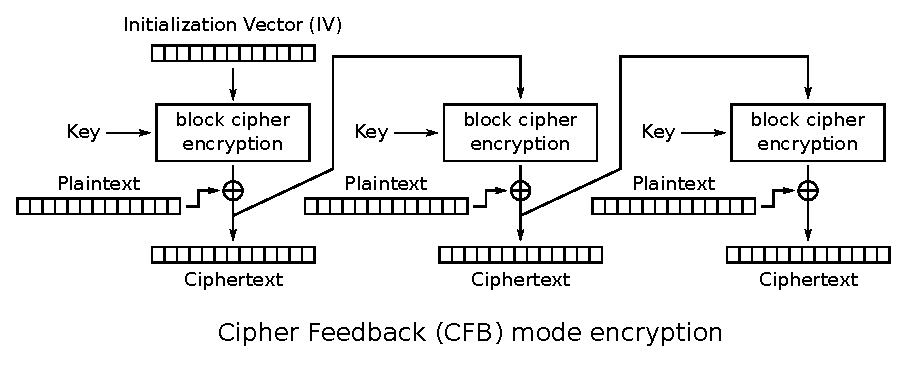
\includegraphics[scale=1]{chapters/chapter_3/CFB.eps}
\end{figure}
\subsection{输出反馈模式(OFB)}
OFB模式与CFB模式极其类似,区别仅在于每组向移位寄存器内的输入为上一组内与明文异或之前的输出。如下图所示(图源wiki):
\begin{figure}[H]
\centering
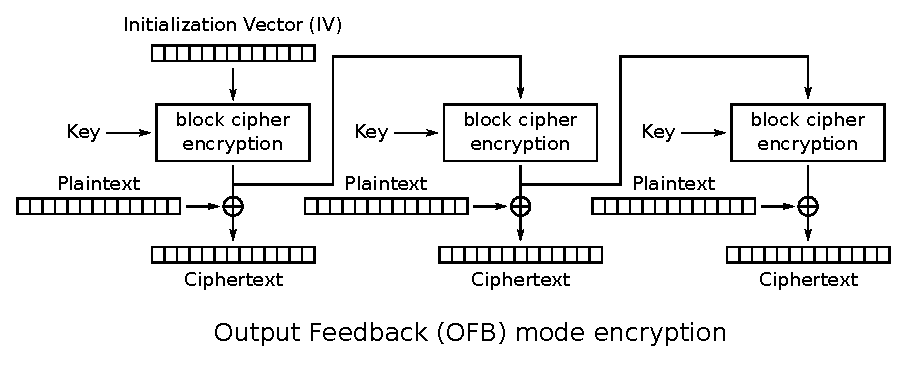
\includegraphics[scale=1]{chapters/chapter_3/OFB.eps}
\end{figure}

从图中可以看到,每组之间传递的数据与明文无关。因此,在OFB中,明文出错只会影响该组的密文,之后的密文都不会被影响。\par
我们如果再仔细看一下OFB的模式图,会发现,事实上,OFB模式把分组密码变成了流密码。真正经过分组密码体系加密的是密钥,而明文则是通过与密钥加密出来的结果异或产生的密文。因此,如果要使OFB模式的安全性高,则要求由分组密码加密出来的密钥为伪随机序列。
\subsection{计数器模式(CTR)}
在借鉴了OFB中本组明文不参与下一组加密的经验之后,引入了CTR模式。在CTR模式中,存在一个计数器函数$f$. 其接受一个初始值,并在每组加密完成后,进行计数,累加到初始值之上。然后每组加密的时候,只需要将该函数的返回值输入分组加密算法中,输出值与当前明文组异或产生密文输出。\par
其过程如图所示(图源wiki):
\begin{figure}[H]
\centering
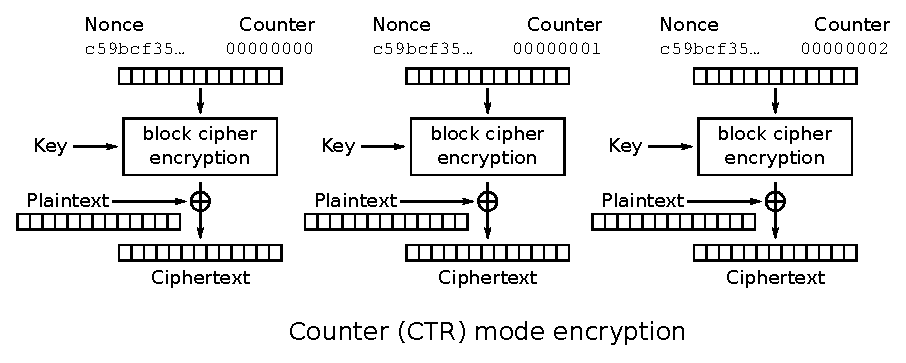
\includegraphics[scale=1]{chapters/chapter_3/CTR.eps}
\end{figure}

根据上图,我们可以发现CTR的独一无二的好处:可以并行加密。其每组加密不需要上组的任何信息,只需要该组对应的计数器值即可。
\section{DES}
接下来,我们讨论的是,在每组内的分组加密算法。\par
DES是最著名的分组密码之一。我们可以先大致地讨论其算法,然后再讨论其一些性质。
\subsection{算法与代码}
DES采用了费斯妥密码的结构,并对它进行了一定的改进。之前我们提到的费斯妥密码,可以改进的地方有其最开始的输入、子密钥、轮函数以及最后的输出。因此,我们分别就上述几个方面来分块解释DES的算法。
\subsubsection{主体:费斯妥密码}
首先,我们介绍DES的主体——费斯妥密码。正如之前说的,费斯妥密码为一个步骤的多轮操作。其核心公式为
\begin{gather}
    L_{i}=R_{i-1}\\
    R_{i}=L_{i-1}\oplus F\pth{R_{i-1}, K_i}
\end{gather}
其中,$L_{i-1}, R_{i-1}$为上一轮输出的左右两半,$L_i, R_i$为本轮输出的左右两半,$F\pth{R_{i-1}, K_i}$为轮函数,$K_i$为本轮的子密钥。\par
此外,从数学上可以证明,费斯妥密码的解密过程的核心公式也是上述公式,只不过使用的密钥的顺序与加密正好相反。\par
DES密码一共进行16轮这样的步骤,并且其输入为64位二进制串,子密钥为48位二进制串,输出为64位二进制串。\par
其C程序代码如下:
\begin{prove}
\begin{verbatim}
bitset<64> round(bitset<64> input, bitset<48> ki)
{
    bitset<64> output;
    bitset<32> previousLeftPart;
    bitset<32> leftPart;
    bitset<32> rightPart;
    
    for (int i = 0; i < 32; i++)
        previousLeftPart[31 - i] = input[63 - i];
    
    for (int i = 0; i < 32; i++)
        leftPart[31 - i] = input[31 - i];
    
    rightPart = previousLeftPart ^ F(leftPart, ki);
    
    for (int i = 0; i < 32; i++)
        output[63 - i] = leftPart[31 - i];
    
    for (int i = 32; i < 64; i++)
        output[63 - i] = rightPart[63 - i];

    return output;
}
\end{verbatim}
\end{prove}
\subsubsection{费斯妥密码的轮函数}
在费斯妥密码的轮函数这里,实际上是采用了SP网络的思想,也就是将轮函数的输入经过S盒的代换来混淆和P盒的置换来扩散。\par
轮函数接受32位的输入和48位的子密钥。首先,将32位的输入扩充成48位的二进制串(可以理解成通过了一个32位到48位的S盒,称为选择扩展运算E),然后将其逐比特与48位的子密钥异或,输出的48位二进制串作为一个48位到32位的S盒的输入。接着,将S盒输出的32位二进制串经过一个P盒(称为置换运算P)输出。\par
这里的48位到32位的S盒实际上是由8个6位到4位的S盒组成。其将输入的48位分组输入,然后再分组输出。\par
因此,轮函数所做的事情有:将32位的输入扩展成48位,进行异或,输入S盒,输入P盒。其C程序代码如下:
\begin{prove}
    \begin{verbatim}
int E[] = {32,  1,  2,  3,  4,  5,
            4,  5,  6,  7,  8,  9,
            8,  9, 10, 11, 12, 13,
           12, 13, 14, 15, 16, 17,
           16, 17, 18, 19, 20, 21,
           20, 21, 22, 23, 24, 25,
           24, 25, 26, 27, 28, 29,
           28, 29, 30, 31, 32,  1};

int S_BOX[8][4][16] = {
    {
        {14,4,13,1,2,15,11,8,3,10,6,12,5,9,0,7},
        {0,15,7,4,14,2,13,1,10,6,12,11,9,5,3,8},
        {4,1,14,8,13,6,2,11,15,12,9,7,3,10,5,0},
        {15,12,8,2,4,9,1,7,5,11,3,14,10,0,6,13}
    },
    {
        {15,1,8,14,6,11,3,4,9,7,2,13,12,0,5,10},
        {3,13,4,7,15,2,8,14,12,0,1,10,6,9,11,5},
        {0,14,7,11,10,4,13,1,5,8,12,6,9,3,2,15},
        {13,8,10,1,3,15,4,2,11,6,7,12,0,5,14,9}
    },
    {
        {10,0,9,14,6,3,15,5,1,13,12,7,11,4,2,8},
        {13,7,0,9,3,4,6,10,2,8,5,14,12,11,15,1},
        {13,6,4,9,8,15,3,0,11,1,2,12,5,10,14,7},
        {1,10,13,0,6,9,8,7,4,15,14,3,11,5,2,12}
    },
    {
        {7,13,14,3,0,6,9,10,1,2,8,5,11,12,4,15},
        {13,8,11,5,6,15,0,3,4,7,2,12,1,10,14,9},
        {10,6,9,0,12,11,7,13,15,1,3,14,5,2,8,4},
        {3,15,0,6,10,1,13,8,9,4,5,11,12,7,2,14}
    },
    {
        {2,12,4,1,7,10,11,6,8,5,3,15,13,0,14,9},
        {14,11,2,12,4,7,13,1,5,0,15,10,3,9,8,6},
        {4,2,1,11,10,13,7,8,15,9,12,5,6,3,0,14},
        {11,8,12,7,1,14,2,13,6,15,0,9,10,4,5,3}
    },
    {
        {12,1,10,15,9,2,6,8,0,13,3,4,14,7,5,11},
        {10,15,4,2,7,12,9,5,6,1,13,14,0,11,3,8},
        {9,14,15,5,2,8,12,3,7,0,4,10,1,13,11,6},
        {4,3,2,12,9,5,15,10,11,14,1,7,6,0,8,13}
    },
    {
        {4,11,2,14,15,0,8,13,3,12,9,7,5,10,6,1},
        {13,0,11,7,4,9,1,10,14,3,5,12,2,15,8,6},
        {1,4,11,13,12,3,7,14,10,15,6,8,0,5,9,2},
        {6,11,13,8,1,4,10,7,9,5,0,15,14,2,3,12}
    },
    {
        {13,2,8,4,6,15,11,1,10,9,3,14,5,0,12,7},
        {1,15,13,8,10,3,7,4,12,5,6,11,0,14,9,2},
        {7,11,4,1,9,12,14,2,0,6,10,13,15,3,5,8},
        {2,1,14,7,4,10,8,13,15,12,9,0,3,5,6,11}
    }
};

int P[] = {16,  7, 20, 21,
           29, 12, 28, 17,
            1, 15, 23, 26,
            5, 18, 31, 10,
            2,  8, 24, 14,
           32, 27,  3,  9,
           19, 13, 30,  6,
           22, 11,  4, 25};

bitset<4> S_boxi(bitset<6> input, int i)
{
    int row = 2 * input[5] + input[0];
    int column = 8 * input[4] + 4 * input[3] + 2 * input[2]
                 + input[1];
    int outputint = S_BOX[i][row][column];
    bitset<4> output(outputint);

    return output;
}
           
bitset<32> S_box(bitset<48> input)
{
    bitset<32> output;
    bitset<6> SiInput[8];

    for (int i = 0; i < 8; i++)
    {
        for (int j = 0; j < 6; j++)
            SiInput[i][5 - j] = input[47 - (j + i * 6)];

        bitset<4> SiOutput = S_boxi(SiInput[i], i);

        for (int j = 0; j < 4; j++)
            output[31 - (j + i * 4)] = SiOutput[3 - j];
    }

    return output;
}
           
bitset<32> F(bitset<32> rightPart, bitset<48> ki)
{
    bitset<32> output;
    bitset<48> expandedInput;

    for (int i = 0; i < 48; i++)
        expandedInput[47 - i] = rightPart[32 - E[i]];

    bitset<48> S_boxInput = expandedInput ^ ki;
    bitset<32> S_boxOutput = S_box(S_boxInput);

    for (int i = 0; i < 32; i++)
        output[31 - i] = S_boxOutput[32 - P[i]];

    return output;
}
    \end{verbatim}
\end{prove}
\subsubsection{费斯妥密码的最初输入}
DES加密算法接受64位明文输入,DES解密算法接受64位密文输入。为了更好地实现扩散性,首先,需要将输入的64位二进制串经过一个P盒。在DES算法中,这个P盒被称作初始置换IP. 随后,将经过置换后的64位二进制串作为费斯妥密码的输入。\par
其C程序代码如下:
\begin{prove}
    \begin{verbatim}
int IP[] = {58, 50, 42, 34, 26, 18, 10, 2,
            60, 52, 44, 36, 28, 20, 12, 4,
            62, 54, 46, 38, 30, 22, 14, 6,
            64, 56, 48, 40, 32, 24, 16, 8,
            57, 49, 41, 33, 25, 17, 9,  1,
            59, 51, 43, 35, 27, 19, 11, 3,
            61, 53, 45, 37, 29, 21, 13, 5,
            63, 55, 47, 39, 31, 23, 15, 7};

bitset<64> getInitialPermutation(bitset<64> input)
{
    bitset<64> initialPermutation;

    for (int i = 0; i < 64; i++)
        initialPermutation[63 - i] = input[64 - IP[i]];

    return initialPermutation;
}
    \end{verbatim}
\end{prove}
\subsubsection{费斯妥密码的最终输出}
之前我们再三强调,费斯妥密码的最后一轮输出后,还要将左右两边互换,也就是最终输出为$\pth{R_{16}, L_{16}}$而非$\pth{L_{16}, R_{16}}$. 此外,为了使DES的加密和解密算法能尽可能复用,我们将输出再经过一个P盒才形成最终的DES的输出。其中,输出时经过的P盒要是输入时P盒的逆,被称为逆初始置换$\mathrm{IP}^{-1}$. 这样的话,我们假设明文为$m$, 密文为$c$, 中间的费斯妥密码部分(包括最后的左右交换),加密为$f(x)$, 解密为$f^{-1}(x)$. 那么,DES加密的过程为
\[c=\mathrm{IP}^{-1}\pth{f\pth{\mathrm{IP}\pth{m}}}\]

而只需要把中间的$f$换成$f^{-1}$:
\begin{align*}
    &\mathrm{IP}^{-1}\pth{f^{-1}\pth{\mathrm{IP}\pth{c}}}\\
    =&\mathrm{IP}^{-1}\pth{f^{-1}\pth{\mathrm{IP}\pth{\mathrm{IP}^{-1}\pth{f\pth{\mathrm{IP}\pth{m}}}}}}\\
    =&\mathrm{IP}^{-1}\pth{f^{-1}\pth{f\pth{\mathrm{IP}\pth{m}}}}\\
    =&\mathrm{IP}^{-1}\pth{\mathrm{IP}\pth{m}}\\
    =&m
\end{align*}
即可实现解密。\par
因此,DES输出包括交换费斯妥密码输出的左右位置,以及通过逆初始置换$\mathrm{IP}^{-1}$. 其C程序代码如下:
\begin{prove}
    \begin{verbatim}
int IP_1[] = {40, 8, 48, 16, 56, 24, 64, 32,
              39, 7, 47, 15, 55, 23, 63, 31,
              38, 6, 46, 14, 54, 22, 62, 30,
              37, 5, 45, 13, 53, 21, 61, 29,
              36, 4, 44, 12, 52, 20, 60, 28,
              35, 3, 43, 11, 51, 19, 59, 27,
              34, 2, 42, 10, 50, 18, 58, 26,
              33, 1, 41,  9, 49, 17, 57, 25};

bitset<64> exchangeLeftAndRight(bitset<64> input)
{
    bitset<64> output;

    for (int i = 0; i < 32; i++)
        output[63 - i] = input[31 - i];

    for (int i = 32; i < 64; i++)
        output[63 - i] = input[95 - i];

    return output;
}

bitset<64> getInversePermutation(bitset<64> input)
{
    bitset<64> output;

    for (int i = 0; i < 64; i++)
        output[63 - i] = input[64 - IP_1[i]];

    return output;
}
    \end{verbatim}
\end{prove}
\subsubsection{密钥的处理}
对于输入的密钥,我们需要让其生成16个子密钥。类似于费斯妥密码,这里的16次生成也是同样的步骤循环16次。但首先,我们需要处理的是DES算法输入的64位密钥。\par
DES算法输入的64位密钥中,通常包含8位奇偶校验位。首先,我们将奇偶校验位去除,得到56位的真正的密钥。然后,再将其通过一个P盒(称为置换选择1:PC\_1),作为接下来生成子密钥的算法的输入。\par
其C程序代码为:
\begin{prove}
\begin{verbatim}
int PC_1[] = {57, 49, 41, 33, 25, 17, 9,
               1, 58, 50, 42, 34, 26, 18,
              10,  2, 59, 51, 43, 35, 27,
              19, 11,  3, 60, 52, 44, 36,
              63, 55, 47, 39, 31, 23, 15,
               7, 62, 54, 46, 38, 30, 22,
              14,  6, 61, 53, 45, 37, 29,
              21, 13,  5, 28, 20, 12,  4};

bitset<56> getKeyPermutation(bitset<64> key)
{
    bitset<56> output;

    for (int i = 0; i < 56; i++)
        output[55 - i] = key[64 - PC_1[i]];

    return output;
}
\end{verbatim}
\end{prove}
\subsubsection{子密钥的生成}
由于DES算法中的费斯妥密码部分一共需要16轮循环,因此共需要16个子密钥。在DES算法中,采用了同一个步骤循环16次的方式生成子密钥。该步骤接受56位二进制串的输入,生成48位的子密钥和56位的输出。其包含两个操作:循环移位和置换选择2。\par
之前我们提到,在DES密码算法中,加密和解密仅有的区别就是子密钥的使用顺序。因此,这种区别就体现在了子密钥生成的算法上。\par
在循环移位步骤中,其接受56位的输入,然后将这56位的二进制串分为左右两个28位的二进制串。并在每一轮中,将这两个二进制串分别循环移位。加密过程是左循环移位,解密过程是右循环移位,并且每一轮移动的位数不同。\par
在循环移位操作完成后,将左右两个二进制串重新拼成一个56位的二进制串作为输出和下一轮操作的输入,同时,再将56位的二进制串经过一个56位到48位的S盒(称为置换选择2: PC\_2), 作为本轮的子密钥。\par
其C程序代码为:
\begin{prove}
\begin{verbatim}
enum ShiftStyle {
    leftShift,
    rightShift
};

int shiftBits[] = {1, 1, 2, 2, 2, 2, 2, 2, 1, 2, 2, 2, 2, 
                    2, 2, 1};
int inverseShiftBits[] = {0, 1, 2, 2, 2, 2, 2, 2, 1, 2, 2, 
                            2, 2, 2, 2, 1};

int PC_2[] = {14, 17, 11, 24,  1,  5,
               3, 28, 15,  6, 21, 10,
              23, 19, 12,  4, 26,  8,
              16,  7, 27, 20, 13,  2,
              41, 52, 31, 37, 47, 55,
              30, 40, 51, 45, 33, 48,
              44, 49, 39, 56, 34, 53,
              46, 42, 50, 36, 29, 32};

bitset<56> shiftKey(bitset<56> key, int round, 
                    ShiftStyle shiftStyle)
{
    bitset<56> output;

    bitset<28> previousLeftPart;
    for (int i = 0; i < 28; i++)
        previousLeftPart[27 - i] = key[55 - i];

    bitset<28> previousRightPart;
    for (int i = 0; i < 28; i++)
        previousRightPart[27 - i] = key[27 - i];

    int *shift;
    switch (shiftStyle)
    {
        case leftShift:
            shift = shiftBits;
            break;
            
        case rightShift:
            shift = inverseShiftBits;
            break;
            
        default:
            break;
    }
    
    bitset<28> leftPart;
    bitset<28> rightPart;
    int shiftBit = shift[round];

    switch (shiftStyle)
    {
        case leftShift:
            for (int i = 0; i < 28; i++)
            {
                leftPart[27 - i] = previousLeftPart[(27 - i
                                     - shiftBit + 28) % 28];
                rightPart[27 - i] = previousRightPart[(27 - i
                                     - shiftBit + 28) % 28];
            }
            break;
            
        case rightShift:
            for (int i = 0; i < 28; i++)
            {
                leftPart[27 - i] = previousLeftPart[(27 - i
                                     + shiftBit + 28) % 28];
                rightPart[27 - i] = previousRightPart[(27 - i
                                     + shiftBit + 28) % 28];
            }
            break;
            
        default:
            break;
    }

    for (int i = 0; i < 28; i++)
        output[55 - i] = leftPart[27 - i];

    for (int i = 28; i < 56; i++)
        output[55 - i] = rightPart[55 - i];

    return output;
}

bitset<48> getSubkey(bitset<56> key, int round, 
                     ShiftStyle shiftStyle)
{
    bitset<48> output;

    for (int i = 0; i < 48; i++)
        output[47 - i] = key[56 - PC_2[i]];

    return output;
}
\end{verbatim}
\end{prove}
\subsubsection{DES加密和解密}
以上就是DES密码的每个组成部分。我们可以把它们组合起来,实现DES的加密和解密。其C程序代码如下:
\begin{prove}
\begin{verbatim}
bitset<64> DES_ENC(bitset<64> plainText, bitset<64> key)
{
    bitset<64> cipher;
    bitset<64> roundInput = getInitialPermutation(plainText);
    bitset<64> roundOutput;
    bitset<56> permutatedKey = getKeyPermutation(key);
    bitset<56> previousShiftOutput = shiftKey(permutatedKey, 0,
                                                 leftShift);
    for (int i = 0; i < 16; i++)
    {
        bitset<48> subkey = getSubkey(previousShiftOutput, i, 
                                        leftShift);
        roundOutput = round(roundInput, subkey);
        roundInput = roundOutput;
        previousShiftOutput = shiftKey(previousShiftOutput, 
                                        i + 1, leftShift);
    }
    cipher = getInversePermutation(
                exchangeLeftAndRight(roundOutput));
    return cipher;
}

bitset<64> DES_DEC(bitset<64> cipher, bitset<64> key)
{
    bitset<64> plainText;
    bitset<64> roundInput = getInitialPermutation(cipher);
    bitset<64> roundOutput;
    bitset<56> permutatedKey = getKeyPermutation(key);
    bitset<56> previousShiftOutput = shiftKey(permutatedKey, 0, 
                                                rightShift);
    for (int i = 0; i < 16; i++)
    {
        bitset<48> subkey = getSubkey(previousShiftOutput, i, 
                                        rightShift);
        roundOutput = round(roundInput, subkey);
        roundInput = roundOutput;
        previousShiftOutput = shiftKey(previousShiftOutput, 
                                        i + 1, rightShift);
    }
    plainText = getInversePermutation(
                    exchangeLeftAndRight(roundOutput));
    return plainText;
}
\end{verbatim}
\end{prove}
\subsection{多重DES}
我们可以看出,DES密码使用了费斯妥密码,并且局部也使用了SP网络,这样使这种分组密码的安全性较高。在几乎30年的大量研究之后,已知对DES的最好的实用攻击仍然只是对密钥空间的穷举搜索。但是,DES使用的密钥在去除奇偶校验位之后的实际长度只有56位,在如今的计算机水平下,变得十分容易破解。在2017年,通过计算机更是创下了在25秒内破解DES的记录。\par
鉴于此,人们选择了多重DES加密。如二重DES加密:使用一个112位的密钥$K$, 将其分为$K_1$和$K_2$两个56位的密钥。如果记$\mathrm{E}_k\pth{m}$为DES的加密过程,$\mathrm{D}_k\pth{m}$为DES的解密过程,那么,其加密过程为
\[\mathrm{E}_{K_1}\pth{\mathrm{E}_{K_2}\pth{m}}\]
解密过程为
\[\mathrm{D}_{K_2}\pth{\mathrm{D}_{K_1}\pth{c}}\]

而如今最常用的是二密钥的三重DES,简称为3DES密码。其使用一个112位的密钥$K$, 将其分为$K_1$和$K_2$两个56位的密钥,其加密过程为
\[\mathrm{E}_{K_1}\pth{\mathrm{D}_{K_2}\pth{\mathrm{E}_{K_1}\pth{m}}}\]
解密过程为
\[\mathrm{D}_{K_1}\pth{\mathrm{E}_{K_2}\pth{\mathrm{D}_{K_1}\pth{c}}}\]
\subsection{结构特性}
除了DES的密钥过短,从数学角度来看,DES密码拥有一些结构特性,也降低了其破解的难度。
\subsubsection{互补特性}
对于二进制串$m$, 如果我们记$\overline{m}$为$m$按位取补,并用$\mathrm{DES}_k\pth{m}$表示通过密钥$k$, 二进制串$m$的DES加密的密文,那么,我们可以证明:
\begin{equation}
\mathrm{DES}_{\overline{k}}\pth{\overline{m}}=\overline{\mathrm{DES}_k\pth{m}}
\end{equation}

因此,在使用穷举搜索破解时,可以使工作量减少一半。假设有一个使用已知明文攻击的攻击者,他可以选择明密文对$\pth{M, C}$和$\pth{\overline{M}, C^*}$. 那么,在所有的$2^{56}$个可能的密钥,也就是$2^{55}$对互补的密钥二进制串中,他只需要每对互补的二进制串中取一个,一共搜索$2^{55}$个密钥。对于每个尝试的密钥$l$, 如果$\mathrm{DES}_{l}\pth{M}=C$或$\overline{C^*}$, 就说明密钥是$l$或$\overline{l}$.
\subsubsection{弱密钥与半弱密钥}
在多重DES加密的过程中,有一些密钥十分危险。比如说弱密钥:
\begin{Definition}
在DES加密的过程中,如果存在一个密钥$w$, 使得
\begin{equation}\label{weakKey}
\mathrm{E}_w\pth{\mathrm{E}_w\pth{m}}=m
\end{equation}

则称$w$为弱密钥。
\end{Definition}

从另一个角度解释公式\ref{weakKey}, 也就是说,
\begin{equation}
\mathrm{E}_w\pth{m}=\mathrm{D}_w\pth{m}
\end{equation}

而我们之前提到,DES密码的加密与解密过程唯一的区别就是子密钥的使用顺序。据此我们可以很容易地构造弱密钥$w$, 也就是使其生成子密钥时加密与解密循环移位的结果相同即可。在56位的密钥中,共有4个弱密钥。\par
此外,还有半弱密钥对
\begin{Definition}
在DES加密的过程中,如果存在一对密钥$w_1, w_2$, 使得
\begin{equation}
\mathrm{E}_{w_1}\pth{\mathrm{E}_{w_2}\pth{m}}=m
\end{equation}

则称$w_1, w_2$为一对半弱密钥。
\end{Definition}

在3DES密码中,如果选取的两个密钥是一对半弱密钥,后果不堪设想。在56位的密钥中,共有6对半弱密钥。
\section{IDEA}
\subsection{符号说明}
在介绍IDEA之前,首先,先介绍一些IDEA加密过程中用到的数学符号。
\begin{itemize}
\item 逐比特异或$\oplus$\par
$m_1\oplus m_2$即将两个16位的二进制串逐比特异或。
\item 模$2^{16}$整数加法$\boxplus$\par
即对于16位二进制数$m_1, m_2$, $m_1\boxplus m_2=\pth{m_1+m_2}\bmod{2^{16}}$.
\item 模$2^{16}+1$整数乘法$\odot$\par
即对于16为二进制数$m_1, m_2$, $m_1\odot m_2=\pth{m_1\cdot m_2}\bmod{\pth{2^{16}+1}}$.\par
这里特别指出,如果$m_1=00\ldots 0$, 应把$m_1$看作$2^{16}$. 这是由于$2^{16}+1=65537$为素数,故由数论知识我们可以知道,模$2^{16}+1$的非零整数乘法构成一个群,即所有非零整数都有逆元。此外,这样也可以保证输出一定不会超过16位。由于$2^{16}+1$为素数,所以如果$\pth{m_1m_2}\bmod{\pth{2^{16}+1}}=0$, 则表明$m_1$或$m_2$必然是$2^{16}+1$的倍数。而$m_1, m_2$均为16位字符串,所以这是不可能的。
\end{itemize}
\subsection{轮结构}
和其他分组密码类似,IDEA也是采用了多次重复轮结构的步骤。其轮结构如图所示(图源wiki):
\begin{figure}[H]
\centering
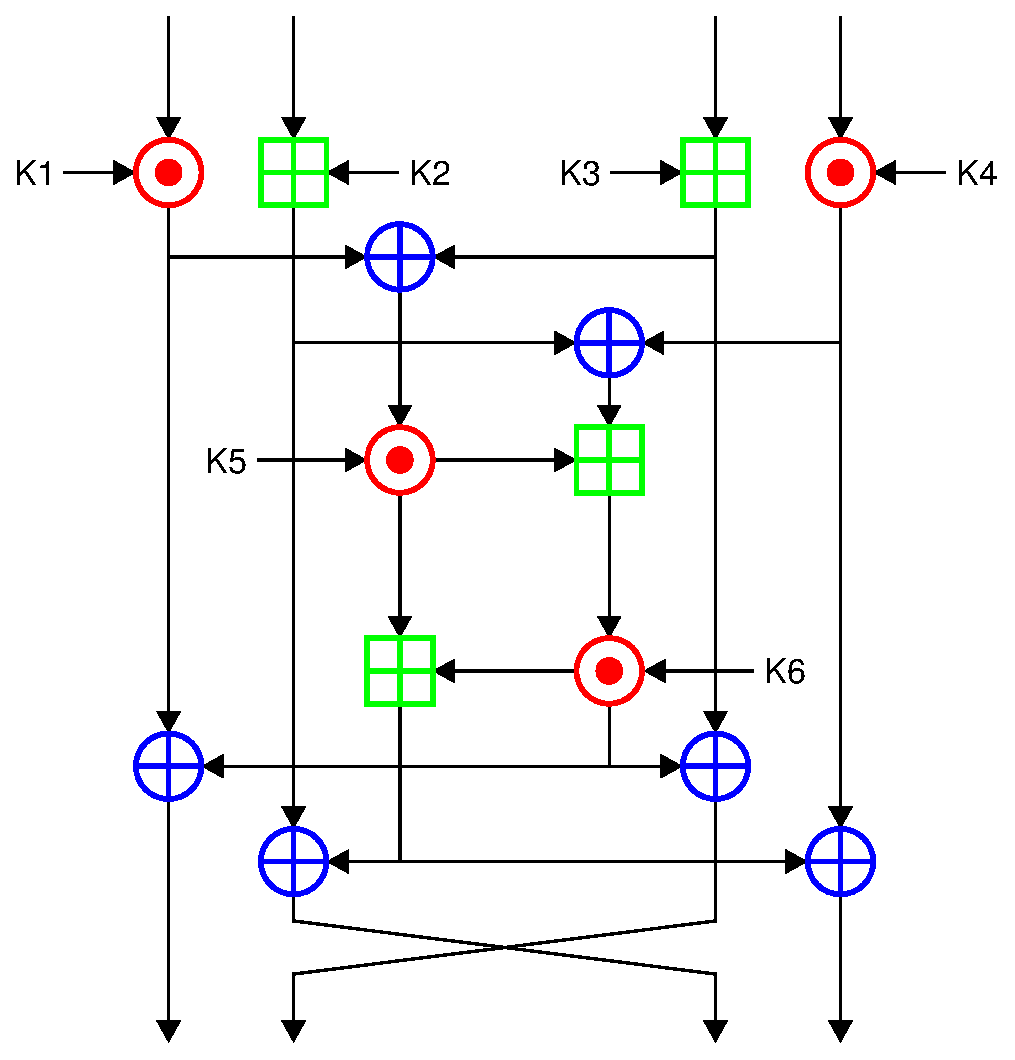
\includegraphics[scale=0.5]{chapters/chapter_3/IDEA_round.eps}
\end{figure}

在每一轮中,一共需要输入6个16位的子密钥,并且输入为4组16位的二进制串,输出也为4组16位的二进制串。
\subsection{加密过程}
IDEA加密算法接受64位明文和128位密钥。对于密钥,将其通过一个子密钥生成器生成48个16位的子密钥用于8轮轮结构,加上6个16位的子密钥用于输出变换。\par
首先,将64位明文分成4组等长的子串,然后输入轮结构中。在经过8轮轮结构后,将输出的结构通过如图所示的输出变换(图源wiki),得到密文。
\begin{figure}[H]
\centering
\includegraphics[scale=0.5]{chapters/chapter_3/IDEA_output.png}
\end{figure}

而子密钥的生成算法则相对比较直接:\par
前8个子密钥$Z_1, Z_2, \ldots, Z_8$直接在加密密钥中依次选取。然后,将加密密钥循环左移$52$位,再依次取接下来的8个子密钥。以此类推,直到52个子密钥全部生成。
\section{AES}
\subsection{输入与输出}
AES密码接受的明文与密钥的长度可独立选择128位、192位或256位。这些选择之间的区别仅仅在于加密运算的轮数以及子密钥的调度不同。但是在AES密码标准中,明文长度固定为128位,密钥长度可以选择为128, 192或256位,分别叫做AES-128, AES-192和AES-256.\par
在处理过程中,我们对明文和密钥进一步分组。AES密码的每个步骤的处理单位是一个“字节”,即8个比特。因此,我们将明文和密钥分成每组长度为8比特的分组,每个8比特的明文分组称为一个“状态”。\par
对于由字节组成的明文,我们第二次进行分组,使其分成4个等长的分组,记明文的每个分组的长度为$N_b$ (在实际操作中明文总是128位,因此$N_b=4$). 此外,我们也记以字节为单位的密钥的长度除以$4$为$N_k$ ($N_k$的可能取值为$4, 6, 8$). 我们如果假定由字节组成的明文是一个长度为$4N_b$的数列$\{M_n\}$, 那么,我们可以按下表的顺序填充分组:
\begin{table}[H]
\centering
\begin{tabular}{c|c|c|c}\hline
$M_0$&$M_4$&$\cdots$&$M_{4N_b-3}$\\\hline
$M_1$&$M_5$&$\cdots$&$M_{4N_b-2}$\\\hline
$M_3$&$M_6$&$\cdots$&$M_{4N_b-1}$\\\hline
$M_4$&$M_7$&$\cdots$&$M_{4N_b}$\\\hline
\end{tabular}
\end{table}

由明文的分组组成的阵列称为状态阵列。在AES的实际过程中,都是对状态阵列进行操作。最终的密文就是从状态序列中,按写入顺序拿出的序列。\par
因此,在加密的输入阶段,我们要做的事是将明文和密钥按字节分组,然后将明文再填入状态阵列中。在加密的输出阶段,就是将密文从状态阵列中读出,再变成以比特为单位的二进制串(但事实上,明文或密文的按字节分组可以直接在填入状态阵列的时候做。因此,我们只需要实现比特串向字节串的转化用于密钥,而不需要实现字节串向比特串的转化)。在解密阶段,我们要做的也是同样的步骤,只不过是明文和密文对调。\par
此环节的C程序代码如下:
\begin{prove}
\begin{verbatim}
void bitToByte(bitset<128> inputBits, bitset<8> outputBytes[64])
{
    for (int byte = 0; byte < 64; byte++)
        for (int bit = 0; bit < 8; bit++)
            outputBytes[byte][bit] = inputBits[8 * byte + bit];
}

void bitToState(bitset<128> input, bitset<8> state[4][4])
{
    for (int column = 0; column < 4; column++)
        for (int row = 0; row < 4; row++)
            for (int bit = 0; bit < 8; bit++)
                state[row][column][bit] = input[32 * column
                                                + 8 * row + bit];
}

void stateToBit(bitset<8> state[4][4], bitset<128> &output)
{
    for (int column = 0; column < 4; column++)
        for (int row = 0; row < 4; row++)
            for (int bit = 0; bit < 8; bit++)
                output[32 * column + 8 * row + bit]
                    = state[row][column][bit];
}
\end{verbatim}
\end{prove}
\subsection{轮函数}
AES的轮函数由4个计算部件组成,分别为字节代换(ByteSub), 行移位(ShiftRow), 列混合(MixColumn), 密钥加(AddRoundKey).
\subsubsection{字节代换}
字节代换可以看作一个128位到128位的S盒。其接受输入状态阵列,然后对状态阵列实现S盒的操作。\par
在C程序实现里,加密过程中,S盒为\verb`bitset<8> S_box[16][16]`; 解密过程中,S盒为\verb`bitset<8> Inv_S_Box[16][16]`. 这两个S盒的值在AES中是固定的,其生成方式可以看后面的数学论证部分。\par
其C程序实现如下:
\begin{prove}
\begin{verbatim}
void SubByte(bitset<8> state[4][4], CryptoMode cryptoMode)
{
    bitset<8> (*crypto_S_box)[16];

    switch (cryptoMode)
    {
        case Enc:
            crypto_S_box = S_box;
            break;
            
        case Dec:
            crypto_S_box = Inv_S_Box;
            break;
            
        default:
            break;
    }
    
    for (int row = 0; row < 4; row++)
        for (int column = 0; column < 4; column++)
        {
            bitset<8> previousValue = *(*(state + row) + column);
            int S_box_row = previousValue[7] * 8
                                + previousValue[6] * 4
                                    + previousValue[5] * 2
                                        + previousValue[4];
            int S_box_column = previousValue[3] * 8
                                + previousValue[2] * 4
                                    + previousValue[1] * 2
                                        + previousValue[0];
            *(*(state + row) + column)
                = crypto_S_box[S_box_row][S_box_column];
        }
}
\end{verbatim}
\end{prove}
\subsubsection{行移位}
在之前处理数据的时候,我们提到把明文分为4组。每组可以看作一行,每行包括$N_b$个字节。\par
所谓行移位,就是将各行进行循环移位,不同的行的位移量不同。第一行不移位,第二行左移$C_1$, 第三行左移$C_2$, 第四行左移$C_3$. $C_1, C_2, C_3$都与$N_b$有关。\par
在解密时,只需要反向循环移位即可。\par
其C程序实现如下:
\begin{prove}
\begin{verbatim}
int shiftBytes[4] = {0, 1, 2, 3};

void ShiftRows(bitset<8> state[4][4], CryptoMode cryptoMode)
{
    for (int row = 0; row < 4; row++)
    {
        bitset<8> previousRow[4];
        for (int column = 0; column < 4; column++)
            previousRow[column] = state[row][column];
        switch (cryptoMode)
        {
            case Enc:
                for (int column = 0; column < 4; column++)
                    state[row][column]
                        = previousRow[(column
                                       - shiftBytes[row] + 4) % 4];
                break;
                
            case Dec:
                for (int column = 0; column < 4; column++)
                    state[row][column]
                        = previousRow[(column
                                       + shiftBytes[row]) % 4];
                break;
                
            default:
                break;
        }
    }
}
\end{verbatim}
\end{prove}
\subsubsection{列混合}
该步骤是对状态阵列的每一列进行变换。为了方便我们理解以及后面的数学论证,我们将这一步理解成矩阵乘法。由于每一列共有4个元素,因此,我们可以把它看作一个四维列向量$(a_0, a_1, a_2, a_3)^{\mathrm{T}}$. 其输出也为4位列向量$(b_0, b_1, b_2, b_3)^{\mathrm{T}}$.\par
在加密过程中,其计算方法为
\begin{equation}
\pth{\begin{array}{c}b_0\\b_1\\b_2\\b_3\end{array}}=\pth{\begin{array}{cccc}02&03&01&01\\01&02&03&01\\01&01&02&03\\03&01&01&02\end{array}}\pth{\begin{array}{c}a_0\\a_1\\a_2\\a_3\end{array}}
\end{equation}

在解密过程中,其计算方法为
\begin{equation}
\pth{\begin{array}{c}a_0\\a_1\\a_2\\a_3\end{array}}=\pth{\begin{array}{cccc}0e&0b&0d&09\\09&0e&0b&0d\\0d&09&0e&0b\\0b&0d&09&0e\end{array}}\pth{\begin{array}{c}b_0\\b_1\\b_2\\b_3\end{array}}
\end{equation}

这里要特别指出的是,在矩阵相乘时,每一项之间的乘法并不是我们平时用到的十进制乘法。这种乘法遵循特定的乘法表。在C程序实现中,我们发现,只需要使用与01, 02, 03, 09, 0b, 0d, 0e的乘法。因此,对于这7个数,我们各有一张长度为256的表,用于与一个字节对应的比特(共$2^8=256$种)相乘($a_0, a_1, a_2, a_3$都是一个字节)的结果。\par
其C程序实现如下:
\begin{prove}
\begin{verbatim}
bitset<8> *M[4][4] = {
    {Mul_02, Mul_03, Mul_01, Mul_01},
    {Mul_01, Mul_02, Mul_03, Mul_01},
    {Mul_01, Mul_01, Mul_02, Mul_03},
    {Mul_03, Mul_01, Mul_01, Mul_02}
};

bitset<8> *Inv_M[4][4] = {
    {Mul_0e, Mul_0b, Mul_0d, Mul_09},
    {Mul_09, Mul_0e, Mul_0b, Mul_0d},
    {Mul_0d, Mul_09, Mul_0e, Mul_0b},
    {Mul_0b, Mul_0d, Mul_09, Mul_0e}
};

void MixColumns(bitset<8> state[4][4], CryptoMode cryptoMode)
{
    bitset<8>* (*crypto_M)[4][4];

    switch (cryptoMode)
    {
        case Enc:
            crypto_M = &M;
            break;
            
        case Dec:
            crypto_M = &Inv_M;
            break;
            
        default:
            break;
    }
    for (int column = 0; column < 4; column++)
    {
        bitset<8> previousColumn[4];
        for (int row = 0; row < 4; row++)
            previousColumn[row] = state[row][column];
        for (int row = 0; row < 4; row++)
        {
            state[row][column] = 0;
            for (int i = 0; i < 4; i++)
                state[row][column]
                    ^= *(*(*(*crypto_M + row) + i)
                        + previousColumn[row].to_ulong());
        }
    }
}
\end{verbatim}
\end{prove}
\subsubsection{密钥加}
在我们输入密钥之后,首先会通过密钥编排算法,得到若干长度为$N_b$的轮密钥。密钥加即为将轮密钥与当前的状态阵列逐比特异或。解密时再次异或即可。\par
其C程序实现如下:
\begin{prove}
\begin{verbatim}
void AddRoundKey(bitset<8> state[4][4], bitset<32> ki[4])
{
    for (int row = 0; row < 4; row++)
        for (int column = 0; column < 4; column++)
            for (int bit = 0; bit < 8; bit++)
                state[row][column][bit]
                    = ki[row][column * 4 + bit]
                        ^ state[row][column][bit];
}
\end{verbatim}
\end{prove}
\subsubsection{轮函数总的步骤}
在每一轮中,对当前的状态阵列,轮函数依次进行字节代换、行移位、列混合和与当前轮密钥的密钥加,最后输出。\par
在最后一轮中,不进行列混合。
\subsection{密钥编排算法}
之前我们讲到,我们输入的密钥会通过密钥编排算法变成若干长度为$N_b$的轮密钥。密钥编排算法分为密钥扩展和轮密钥选取两个部分。\par
考虑到每个轮密钥长度都为$N_b$, 假设我们需要进行$N_r$轮,则一共需要$N_b\pth{N_r+1}$长度的密钥。因此,我们首先需要将输入的密钥扩展成对应长度的扩展密钥。\par
然后,第一轮轮密钥取扩展密钥的第一个$N_b$长度个字,第二轮轮密钥取接下来的$N_b$长度个字,以此类推。\par
\subsubsection{密钥扩展算法}
在密钥扩展算法中,我们需要用到$N_r$个轮常数\verb`Rcon`,以及一些辅助工作,如对密钥的循环移位\verb`RotWord`和对密钥的替换(使用的S盒与之前的是同一个)\verb`SubWord`. 此外,对于不同的$N_r$, 密钥扩展算法也不同。\par
这里以AES-128为例,其C程序代码如下:
\begin{prove}
\begin{verbatim}
bitset<32> Rcon[10] = {0x01000000, 0x02000000, 0x04000000,
0x08000000, 0x10000000, 0x20000000, 0x40000000, 0x80000000,
0x1b000000, 0x36000000};

bitset<32> RotWord(bitset<32> input)
{
    bitset<32> output;

    for (int i = 0; i < 32; i++)
        output[i] = input[(i - 8 + 32) % 32];

    return output;
}

bitset<32> SubWord(bitset<32> input)
{
    bitset<32> output;
    
    for (int byte = 0; byte < 4; byte++)
    {
        int row = input[8 * byte + 7] * 8
                    + input[8 * byte + 6] * 4
                        + input[8 * byte + 5] * 2
                            + input[8 * byte + 4];
        int column = input[8 * byte + 3] * 8
                        + input[8 * byte + 2] * 4
                            + input[8 * byte + 1] * 2
                                + input[8 * byte];
        bitset<8> value = S_box[row][column];
        for (int bit = 0; bit < 8; bit++)
            output[8 * byte + bit] = value[bit];
    }
    
    return output;
}

void KeyExpansion(bitset<8> *key, bitset<32> *w)
{
    int Nk = 4;
    int Nr = 10;
    
    for (int word = 0; word < Nk; word++)
        for (int byte = 0; byte < 4; byte++)
            for (int bit = 0; bit < 4; bit++)
                w[word][4 * byte + bit] = key[byte][bit];

    for (int word = Nk; word < 4 * (Nr + 1); word++)
    {
        bitset<32> tmp = w[word - 1];
        if (!word % Nk)
            tmp = SubWord(RotWord(tmp)) ^ Rcon[word / Nk];
        w[word] = w[word - Nk] ^ tmp;
    }
}
\end{verbatim}
\end{prove}
\subsection{总的加解密过程}
\subsubsection{加密过程}
首先,将明文写入状态阵列,密钥变成字节串。然后,求出扩展密钥。接着,对前4个密钥使用密钥加算法。然后,在进行10轮的字节替换、行移位、列混合、密钥加,其中最后一轮不进行列混合。最后,将此时的状态阵列读出为密文。\par
其C程序代码如下:
\begin{prove}
\begin{verbatim}
bitset<128> AES_128_ENC(bitset<128> plainText, bitset<128> key)
{
    bitset<128> cipher;
    
    bitset<8> state[4][4];
    bitToState(plainText, state);
    
    bitset<8> keys[16];
    bitToByte(key, keys);
    
    bitset<32> expanedKeys[44];
    KeyExpansion(keys, expanedKeys);
    
    bitset<32> subkeys[4];
    for (int i = 0; i < 4; i++)
        subkeys[i] = expanedKeys[i];
    AddRoundKey(state, subkeys);
    
    for (int round = 0; round < 9; round++)
    {
        SubByte(state, Enc);
        ShiftRows(state, Enc);
        MixColumns(state, Enc);
        for (int i = 0; i < 4; i++)
            subkeys[i] = expanedKeys[i + 4 + round * 4];
        AddRoundKey(state, subkeys);
    }
    
    SubByte(state, Enc);
    ShiftRows(state, Enc);
    for (int i = 0; i < 4; i++)
        subkeys[i] = expanedKeys[i + 40];
    AddRoundKey(state, subkeys);
    
    stateToBit(state, cipher);

    return cipher;
}
\end{verbatim}
\end{prove}
\subsubsection{解密算法}
首先,将密文写入状态阵列,密钥变成字节串。然后,求出扩展密钥。接着,对最后4个密钥使用密钥加算法。然后,在进行10轮的字节替换、行移位、密钥加、列混合,其中最后一轮不进行列混合。最后,将此时的状态阵列读出为明文。\par
解密与加密的区别在于:轮密钥的使用顺序恰好相反(但每一轮内的顺序是相同的)。\par
其C程序代码如下:
\begin{prove}
\begin{verbatim}
bitset<128> AES_128_DEC(bitset<128> cipher, bitset<128> key)
{
    bitset<128> plainText;
    
    bitset<8> state[4][4];
    bitToState(cipher, state);
    
    bitset<8> keys[16];
    bitToByte(key, keys);
    
    bitset<32> expanedKeys[44];
    KeyExpansion(keys, expanedKeys);
    
    bitset<32> subkeys[4];
    for (int i = 0; i < 4; i++)
        subkeys[i] = expanedKeys[40 + i];
    AddRoundKey(state, subkeys);
    
    for (int round = 0; round < 9; round++)
    {
        SubByte(state, Dec);
        ShiftRows(state, Dec);
        MixColumns(state, Dec);
        for (int i = 0; i < 4; i++)
            subkeys[i] = expanedKeys[i + 36 - round * 4];
        AddRoundKey(state, subkeys);
    }
    
    SubByte(state, Dec);
    ShiftRows(state, Dec);
    for (int i = 0; i < 4; i++)
        subkeys[i] = expanedKeys[i];
    AddRoundKey(state, subkeys);
    
    stateToBit(state, plainText);

    return plainText;
}
\end{verbatim}
\end{prove}
\subsection{数学基础}
\subsubsection{有限域$\GF\pth{2^8}$}
我们之前在讲流密码的时候提到过有限域$\GF\pth{2}$. 在这里,我们就要正式地引入域的概念:\par
所谓域,就是可交换的除环。更确切地说:
\begin{Definition}
对于集合$F$和它上面的两个运算$+, \cdot$, 如果满足如下性质:
\begin{enumerate}
    \item 加法和乘法的封闭性\par
    $\forall a, b\in F, a+b\in F, a\cdot b\in F$
    \item 加法和乘法的结合律\par
    $\forall a, b, c\in F, \pth{a+b}+c=a+\pth{b+c}, \pth{a\cdot b}\cdot c=a\cdot\pth{b\cdot c}$
    \item 加法和乘法的交换律\par
    $\forall a, b\in F, a+b=b+a, a\cdot b=b\cdot a$
    \item 乘法对加法的分配率\par
    $\forall a, b, c\in F, a\cdot\pth{b+c}=a\cdot b+a\cdot c$
    \item 加法单位元\par
    $\exists a\in F, \mathrm{s.t.}\, \forall b\in F, a+b=b+a=b$\par
    常将加法单位元$a$记作$0$
    \item 乘法单位元\par
    $\exists a\in F, \mathrm{s.t.}\, \forall b\in F\text{且}b\neq 0, a\cdot b=b\cdot a=b$\par
    常将乘法单位元$a$记作$1$
    \item 加法逆元\par
    $\forall a\in F,\exists -a\in F, \mathrm{s.t.}\, a+\pth{-a}=\pth{-a}+a=0$
    \item 乘法逆元\par
    $\forall a\in F\text{且}a\neq 0, \exists a^{-1}\in F, \mathrm{s.t.}\, a\cdot a^{-1}=a^{-1}\cdot a=0$
\end{enumerate}
则称$F$和它上面的两个运算$+, \cdot$构成一个域。
\end{Definition}

如果$F$内的元素个数有限,为$n$个,则称$F$为有限域,记作$\GF\pth{n}$. 在AES中,我们主要研究有限域$\GF\pth{2^8}$.\par
熟悉抽象代数的同学可能会知道,对于任意素数$p$和正整数$n$, 所有有限域$\GF\pth{p^n}$都是同构的。因此,我们可以使用一个尽可能简单的表示方法来研究$\GF\pth{2^8}$.\par
我们考虑集合$\ext F=\brace{\sum_{i=0}^7a_ix^i\mid a_i\in\GF\pth{2}}$为一个多项式的集合。我们想通过定义其上的加法与乘法使其变成一个$\GF\pth{2^8}$. 这时,就需要我们之前提到的$\GF\pth{2}$上的多项式。为了方便叙述,我们记$G$为$\GF\pth{2}$上的多项式组成的集合,定义$\oplus$和$\odot$为$G$上的加法与乘法,$+$和$\cdot$为$F$上的加法与乘法。\par
如果定义其元素加法为:$\ext\forall p_1=\sum_{i=0}^7a_ix^i\in F, p_2=\sum_{i=0}^7b_ix^i\in F$:
\begin{equation}
p_1+p_2=\sum_{i=0}^7\pth{a_i+b_i}x^i
\end{equation}
其中$a_i+b_i$是$\GF\pth{2}$上的加法,也就是模2加法,或者说是异或。因此,$F$上的加法与$G$上的加法相同。\par
而为了定义其元素乘法,首先引入一个8次不可约多项式
\begin{equation}
m\pth{x}=x^8+x^4+x^3+x+1
\end{equation}

同时,定义$G$上的取模运算为:对于$p_1, p_2\in G$, 如果存在多项式$q\in G, r\in G$, 使得$p_1=q\odot p_2\oplus r$, 且$r$的次数低于$p_2$, 则记作$p_1\bmod{p_2}=r$.\par
接着,我们就可以定义$F$上的乘法为:$\ext\forall p_1=\sum_{i=0}^7a_ix^i\in F, p_2=\sum_{i=0}^7b_ix^i\in F$:
\begin{equation}
p_1\cdot p_2= \pth{p_1\odot p_2}\bmod{m\pth{x}}
\end{equation}

可以证明,$F$对$+, \cdot$构成一个有限域$\GF\pth{2^8}$.\par
此外,我们还需要在$F$上定义一个一元运算,称为$x$乘法:对于$p\in F$, 记
\begin{equation}
\mathrm{xtime}\pth{p}=x\cdot p
\end{equation}

这里需要强调的是,虽然我们用多项式来表示$\GF\pth{2^8}$, 但这并不意味着$\GF\pth{2^8}$的元素就是多项式。我们不在意它的元素是什么,我们关注的是它具有$2^8$个元素,并且它上面的乘法和加法表符合我们之前利用多项式定义的乘法和加法表。
\subsubsection{$\GF\pth{2^8}$上的多项式}
类似于我们之前在流密码中讲到的$\GF\pth{2}$上的多项式,在我们定义了$\GF\pth{2^8}$的加法与乘法之后,就可以定义$\GF\pth{2^8}$上的多项式了。但是在AES中,与$\GF\pth{2}$上的多项式不同的是,$\GF\pth{2^8}$上的多项式为系数属于$\GF\pth{2^8}$且次数小于4的多项式。即集合$\ext\brace{\sum_{i=0}^3a_ix^i\mid a_i\in\GF\pth{2^8}}$.\par
同时,我们定义$\GF\pth{2^8}$上的多项式的模$x^4+1$乘法$\otimes$. 即:
\begin{equation}
p_1\otimes p_2=\pth{p_1\cdot p_2}\bmod{\pth{x^4+1}}
\end{equation}
其中$\cdot$是$\GF\pth{2^8}$上的多项式的普通乘法。\par
此外,如果我们假设$\ext p_1=\sum_{i=0}^3a_ix^i, p_2=\sum_{i=0}^3b_ix^i$, 那么
\begin{align*}
p_1\cdot p_2&=\sum_{i=0}^3\sum_{j=0}^3a_ib_jx^{i+j}\\
&=a_0b_0+\pth{a_0b_1+a_1b_0}x+\pth{a_0b_2+a_1b_1+a_2b_0}x^2+\pth{a_0b_3+a_1b_2+a_2b_1+a_3b_0}x^3\\
&+\pth{a_1b_3+a_2b_2+a_3b_1}x^4+\pth{a_2b_3+a_3b_2}x^5+a_3b_3x^6
\end{align*}

如果我们记$t_{ij}$为$p_1\cdot p_2$中$x^i$的系数中,$b_j$前面的系数(如$t_{00}=a_0, t_{10}=a_1$),那么
\begin{align*}
p_1\otimes p_2&=\pth{\sum_{i=0}^6\pth{\sum_{j=0}^3t_{ij}b_j}x^i}\bmod{\pth{x^4+1}}\\
&=\sum_{i=0}^3\pth{\sum_{j=0}^3t_{ij}b_j}x^i+\sum_{j=4}^6\pth{\sum_{j=0}^3t_{ij}b_j}\pth{x^j\bmod{\pth{x^4+1}}}
\end{align*}

如果记$\ext x^i\bmod{\pth{x^4+1}}=\sum_{j=0}^3{\alpha_{ij}x^j}$, 同时如果我们假设$\ext p_1\otimes p_2=\sum_{i=0}^3c_ix^i$, 那么
\begin{align*}
\sum_{i=0}^3c_ix^i&=\sum_{i=0}^3\pth{\sum_{j=0}^3t_{ij}b_j}x^i+\sum_{k=4}^6\pth{\sum_{m=0}^3t_{km}b_m}\pth{\sum_{l=0}^3{\alpha_{kl}x^l}}\\
&=\sum_{i=0}^3\pth{\sum_{j=0}^3t_{ij}b_j}x^i+\sum_{l=0}^3\pth{\sum_{k=4}^6\pth{\sum_{m=0}^3t_{km}b_m}\alpha_{kl}}x^l\\
&=\sum_{i=0}^3\pth{\sum_{j=0}^3\pth{t_{ij}+\sum_{k=4}^6t_{kj}\alpha_{ki}}b_j}x^i
\end{align*}

因此
\begin{equation}
c_i=\sum_{j=0}^3\pth{t_{ij}+\sum_{k=4}^6t_{kj}\alpha_{ki}}b_j
\end{equation}

注意到这个式子中,$t_{ij}, t_{kj}, \alpha_{ki}$都与$p_2$无关,因此可以提前算出来。从而,我们可以得到:
\begin{theorem}
对于多项式$p_1=a_0+a_1x+a_2x^2+a_3x^3$和$p_2=b_0+b_1x+b_2x^2+b_3x^3$, 若$p_1\otimes p_2=c_0+c_1x+c_2x^2+c_3x^3$, 则
\begin{equation}
\pth{\begin{array}{c}c_0\\c_1\\c_2\\c_3\end{array}}=\pth{\begin{array}{cccc}a_0&a_3&a_2&a_1\\a_1&a_0&a_3&a_2\\a_2&a_2&a_0&a_3\\a_3&a_2&a_1&a_0\end{array}}\pth{\begin{array}{c}b_0\\b_1\\b_2\\b_3\end{array}}
\end{equation}
这里矩阵里元素的乘法是$\GF\pth{2^8}$上的乘法。
\end{theorem}

同时还有一个推论:
\begin{theorem}
$\GF\pth{2^8}$上的多项式$a_3x^3+a_2x^2+a_1x+a_0$是模$x^4+1$可逆的,当且仅当矩阵
\[\pth{\begin{array}{cccc}a_0&a_3&a_2&a_1\\a_1&a_0&a_3&a_2\\a_2&a_2&a_0&a_3\\a_3&a_2&a_1&a_0\end{array}}\]
在$\GF\pth{2^8}$上是可逆的。
\end{theorem}
\subsubsection{AES加密过程}
在AES加密的过程中,我们将长度为128个比特的明文分成了4行$N_b=4$列的状态阵列。每个阵列元素为一个长度为8比特的字节。因此,一共有$2^8=256$种字节。所以,我们可以将一个字节看作一个$\GF\pth{2^8}$中的元素。\par
加密过程中的字节代换分为两步:
\begin{enumerate}
    \item 将字节看作$\GF\pth{2^8}$上的元素,将其映射到自己的乘法逆元。全0字节映射到自己。
    \item 接着,对字节作以下$\GF\pth{2}$上的运算,输出$\pth{y_0, y_1, \ldots ,y_7}$:
    \begin{equation}
    \pth{\begin{array}{c}y_0\\y_1\\y_2\\y_3\\y_4\\y_5\\y_6\\y_7\end{array}}=\pth{
\begin{array}{cccccccc}
1     & 0     & 0     & 0     & 1     & 1     & 1     & 1 \\
1     & 1     & 0     & 0     & 0     & 1     & 1     & 1 \\
1     & 1     & 1     & 0     & 0     & 0     & 1     & 1 \\
1     & 1     & 1     & 1     & 0     & 0     & 0     & 1 \\
1     & 1     & 1     & 1     & 1     & 0     & 0     & 0 \\
0     & 1     & 1     & 1     & 1     & 1     & 0     & 0 \\
0     & 0     & 1     & 1     & 1     & 1     & 1     & 0 \\
0     & 0     & 0     & 1     & 1     & 1     & 1     & 1 \\
\end{array}%
}\pth{\begin{array}{c}x_0\\x_1\\x_2\\x_3\\x_4\\x_5\\x_6\\x_7\end{array}}+\pth{\begin{array}{c}1\\1\\0\\0\\0\\1\\1\\0\end{array}}
    \end{equation}
\end{enumerate}
在解密过程中,将上述的矩阵换为其逆矩阵即可。\par
对于加密过程中的列混合:\par
由于明文被分为4组,每组看作一行,那么对于每列来说,都含有四个元素,且每个元素都属于$\GF\pth{2^8}$. 因此,可以将每列看作$\GF\pth{2^8}$上的多项式。接着,记
\begin{equation}
c\pth{x}=\pth{03}_{16}x^3+\pth{01}_{16}x^2+\pth{01}_{16}x+\pth{02}_{16}
\end{equation}
其中$\pth{03}_{16}, \pth{01}_{16}, \pth{02}_{16}$都是用两个16进制数表示的8比特二进制串。\par
然后,对于每列对应的$\GF\pth{2^8}$上的多项式,将其与$c\pth{x}$作$\GF\pth{2^8}$上多项式的模$x^4+1$乘法$\otimes$来输出。利用之前的讨论,我们可以得到
\begin{equation}
\pth{\begin{array}{c}b_0\\b_1\\b_2\\b_3\end{array}}=\pth{\begin{array}{cccc}02&03&01&01\\01&02&03&01\\01&01&02&03\\03&01&01&02\end{array}}\pth{\begin{array}{c}a_0\\a_1\\a_2\\a_3\end{array}}
\end{equation}
其中的运算作$\GF\pth{2^8}$上的运算。\par
而通过数学上的计算可知,如果记
\begin{equation}
d\pth{x}=\pth{0B}_{16}x^3+\pth{0D}_{16}x^2+\pth{09}_{16}x+\pth{0E}_{16}
\end{equation}

则在解密运算中,将每列与$d(x)$作$\GF\pth{2^8}$上多项式的模$x^4+1$乘法$\otimes$来输出即可。类似地,也有一个对应的矩阵
\begin{equation}
\pth{\begin{array}{c}a_0\\a_1\\a_2\\a_3\end{array}}=\pth{\begin{array}{cccc}0e&0b&0d&09\\09&0e&0b&0d\\0d&09&0e&0b\\0b&0d&09&0e\end{array}}\pth{\begin{array}{c}b_0\\b_1\\b_2\\b_3\end{array}}
\end{equation}

对于密钥编排算法:\par
密钥编排算法中用到了轮常数\verb`Rcon`. 对于\verb`Rcon`的第$i$个元素的形式为$\pth{\pth{rc_i}_{16}, 00, 00, 00}$, 其算法为
\begin{equation}
rc_i=2\cdot rc_{i-1}
\end{equation}
其中$\cdot$为$\GF\pth{2^8}$中的乘法,$rc_0=\pth{01}_{16}$.
% !TEX root = ../../现代密码学简介.tex
\chapter{公钥密码}
\section{简介}
之前我们讲到,最安全的密码体系是一次一密。但是,由于其需要用安全信道传输的密钥长度至少于明文一样长,并且一个密钥只能用一次,因此,与其将密钥传输,不如将明文传输。所以,一次一密的缺陷也十分明显。为了解决这一问题,之前我们采取的方法是使用各种手法,包括流密码以及分组密码等,来缩短密钥的长度。而公钥密码则提供了另一种不同的思路:减弱对安全信道的需求。其基本思想为:
\begin{enumerate}
	\item 由解密方生成一对密钥,称为公钥(记作$SK$)和私钥(记作$PK$)。
	\item 解密方将公钥传送给加密方(不需要通过安全信道)。
	\item 加密方利用公钥加密明文,传递给解密方。
	\item 解密方利用私钥解密密文。
\end{enumerate}

要在实践中实现这个思想,我们得满足:
\begin{itemize}
	\item 生成公钥、密钥对的算法较容易
	\item 用公钥加密明文的算法较容易
	\item 用密钥解密密文的算法较容易
	\item 由公钥不能(或者很难)得到对应的密钥
	\item 由密文和公钥不能(或者很难)得到对应的明文
	\item 公钥、私钥可交换。即:
	\begin{equation}
	\D{PK}{\E{SK}{m}} = \D{SK}{\E{PK}{m}}
	\end{equation}
\end{itemize}

此外,公钥密码体系还有一个重要的特点是,其安全性基于数论知识,而非类似于分组密码的代换与替换。并且,在之后的算法细节中我们会了解到,公钥密码体系的算法比对称密码体系的算法要慢许多。同时,由于并非一次一密,因此其安全性从本质上说并不比对称密码体系高。\par
公钥密码体系也称为非对称密码体系,因为用于加密的公钥不能解密其密文。\par
同时,公钥密码除了解决了密钥分配问题,即对安全信道的需求问题,其还解决了另外一个问题:数字签名问题。即,在以往的对称加密体系中,我们无法得知收到的密文是否来自于我们选择的加密方。
\input{chapters/chapter_5/哈希算法}
% !TEX root = ../../现代密码学简介.tex
\chapter{消息验证码}
\section{简介}
通过上一章的介绍,我们掌握了一个用于验证消息完整性的强大工具:哈希函数。通过比较发送者发送的摘要与接收者计算的摘要,接收者可以判断消息是否在传递过程中受到篡改。但是,这仅仅是第一步。在消息验证的过程中,还有一个非常重要的目的:在确定消息完整性的同时,确定消息发送自期望的发送者。因此,我们引入一个新的工具:消息验证码(Message Authentication Code, MAC).\par
在之前提到安全协议的时候,我们知道,密钥交换协议可以确保消息发送自期望的发送者。但是,密钥交换协议却不能确定消息的完整性。那么,如何同时做到确定消息的完整性,和确定消息发送自期望的发送者呢?\par
在之后提到的安全协议中,我们可以了解到,通过某些协议可以确保消息发自期望的发送者,那么换个角度说,如果接收者能确定消息的发送者和自己使用的是相同的密钥,那么也就能确定消息的发送者是期望的发送者。因此,我们可以结合密钥和之前提到的哈希函数的基本概念,从而提出MAC算法$C_K(m)$的基本概念:
\begin{itemize}
	\item 该算法适用于任意长度的消息$m$
	\item 算法使用一个密钥$K$
	\item 该算法的输出$C_K(m)$是固定长的
	\item 由输入$m$和密钥$K$求得输出$C_K(m)$的过程较容易
	\item 由输出$C_K(m)$反求得输入$m$或密钥$K$的过程是不可行的,或者是难以计算的
	\item 给定$x$, 难以求得$y$, 使得$C_K(x)=C_K(y)$
	\item 难以求得任何一对$\pth{x, y}$, 使得$C_K(x)=C_K(y)$
\end{itemize}

我们可以看到,MAC算法的设计准则和哈希算法的设计准则几乎一致,只是MAC算法还需要一个密钥。此外,MAC算法的输出称为\textbf{标签}(tag).\par
发送方通过密钥$K$, 使用MAC算法对要传递的消息$m$进行处理,得到标签$t$, 将$\pth{m, t}$发送给接收者。接收方接收到$\pth{m', t}$后,通过与发送方共享的密钥$K$, 使用同样的MAC算法对接收到的消息$m'$进行处理,得到标签$t'$. 如果$t'=t$, 那么既说明了发送方发送的消息并没有得到篡改,也说明了发送方与自己使用的是同一个密钥,也就是消息的发送方是期待的发送方。\par
上述过程虽然并不是真的符合认证加密的过程,但是讲述了MAC的基本思想。\par
MAC最主要的两个部分,一个是密钥,一个是类似哈希函数的基本概念。因此,MAC主要的实现方法,也分为两类:基于分组密码,与基于哈希函数。
\section{基于分组密码的MAC算法}
\subsection{CBC-MAC}
我们之前在分组密码中提到,分组密码有许多运行模式。CBC-MAC就是基于密码分组连接模式(CBC)的MAC算法。其也被称为数据认证算法(Data Authentication Algorithm). 但是由于其安全性欠佳,因此已被淘汰。\par
假设要传递的消息为$M$, 密钥为$K$, 分组密码加密算法为$\E{k}{m}$, 其分组长度为$b$比特。\par
CBC-MAC的过程如下:
\begin{enumerate}
	\item 填充\par
	将消息$M$通过在末尾补`0'填充为长度是$b$的整数倍$nb$的二进制串$M'$, 并将其分为$n$个长度为$b$比特的二进制串$m_1, m_2, \ldots, m_n$.
	\item 加密\par
	采用以下公式进行加密:
	\begin{align*}
	&O_1=\E{K}{m_1}\\
	&O_{i}=\E{K}{O_{i-1}\oplus m_{i}},\quad i=2, 3,\ldots, n
	\end{align*}
	\item 输出\par
	CBC-MAC的输出为$b$比特二进制串$O_n$
\end{enumerate}

从本质上来说,这个算法就是一个初始值$\mathrm{IV}=0$的CBC模式分组加密算法,取其最后一个分组的输出。\par
对于固定长度的消息来说,如果使用的分组加密算法是安全的,那么CBC-MAC也是安全的。但是,对于长度不固定的消息来说,这是不安全的。
\subsection{CMAC}
CMAC是NSIT推荐的基于分组加密算法的MAC算法。\par
假设要传递的消息为$M$, 密钥为$K$, 分组密码加密算法为$\E{k}{m}$, 其分组长度为$b$比特。\par
CMAC分为两个步骤:生成子密钥与输出标签。
\subsubsection{生成子密钥}
对于密钥$K$, 采用下面的算法将其生成为两个长度为$b$比特的子密钥$K_1, K_2$
\begin{enumerate}
	\item 计算$b$位二进制数$K_0=\E{K}{0}$
	\item 记$B_0$为$K_0$表示成二进制数时的最高位(第$b$位)。\par
	如果$B_0=0$, 则$K_1=K_0\ll 1$, 其中$x\ll 1$表示将二进制串$x$左移一个比特;\par
	如果$B_0=1$, 则$K_1=\pth{K_0\ll 1}\oplus C$, 其中
	\[C=\begin{dcases}\pth{1B}_{16}&b=64\\\pth{87}_{16}&b=128\\\pth{425}_{16}&b=256\end{dcases}\]
	\item 记$B_1$为$K_1$表示成二进制数时的最高位。\par
	如果$B_1=0$, 则$K_2=K_1\ll 1$.\par
	如果$B_1=1$, 则$K_2=\pth{K_1\ll 1}\oplus C$
\end{enumerate}
\subsubsection{输出标签}
CMAC采用如下算法产生$b$比特的标签:
\begin{enumerate}
	\item 将$M$从头开始分为$n$个子串$m_1, m_2, \ldots, m_n$. 其中$m_1, m_2,\ldots, m_{n-1}$的长度均为$b$比特,$m_n$的长度不大于$b$比特。
	\item 如果$m_n$的长度是$b$比特,那么$m_n'=K_1\oplus m_n$.\par
	如果$m_n$的长度小于$b$比特,那么先在其后补一位`1', 然后一直补`0'直到其长度达到$b$比特的二进制串$m_n''$, 然后$m_n'=K_2\oplus m_n''$.
	\item 采用如下公式加密:
	\begin{align*}
	&O_1=\E{K}{m_1}\\
	&O_{i}=\E{K}{O_{i-1}\oplus m_{i}},\quad i=2, 3,\ldots, n\\
	&O_n=\E{K}{O_{n-1}\oplus m_n'}
	\end{align*}
	\item 输出\par
	CMAC的输出为$b$比特二进制串$O_n$
\end{enumerate}
\section{基于哈希函数的MAC算法}
除了基于分组密码的MAC算法,还有一种是基于哈希函数的MAC算法,称为HMAC.\par
HMAC需要一个哈希函数$H(x)$, 根据我们上一章的记号,假设其输出为$b$比特,输入被处理为$v$比特的块。同时,HMAC还需要一个密钥$K$. 对$K$的长度有如下要求:
\begin{itemize}
\item $K$的长度不建议小于$b$比特。
\item $K$的长度如果大于$v$比特,那么就对$K$进行哈希得到$b$比特长的串$H\pth{K}$作为实际使用的密钥$K$
\end{itemize}

通过上述操作,密钥$K$的长度被控制在不大于$v$比特。接着,在二进制串$K$的尾部填充`0'使得其长度达到$v$比特的新串$K'$.\par
接下来需要定义两个串$\mathrm{ipad}$和$\mathrm{opad}$:
\begin{itemize}
	\item $\mathrm{ipad}$是将十六进制串$36$重复多次得到的长度为$v$的二进制串
	\item $\mathrm{opad}$是将十六进制串$5C$重复多次得到的长度为$v$的二进制串
\end{itemize}

那么,HMAC算法的输出$C_K(m)$的定义为
\begin{equation}
	C_K(m)=H\pth{K'\oplus\mathrm{opad}\parallel H\pth{K'\oplus\mathrm{ipad}\parallel m}}
\end{equation}
其中$x\parallel y$代表将二进制串$y$级联在$x$尾部。
\section{基于全域哈希的MAC算法}
基于全域哈希(Universal hashing)的MAC算法,简称为UMAC. 它的特点是,对于每一次求MAC的消息,其采用的哈希函数是不同的。也就是对于同一个消息,多次求MAC的结果并不相同。现在最常用的UMAC算法,就是Poly1305, 其也被称为目前处于顶尖水平的MAC算法。这种算法运算速度极快,安全性也较高。下面就介绍一下该算法。
\subsection{Poly1305}
该算法接收任意长度的消息$M$,一个256比特的密钥$K$, 输出为128比特的标签。该算法要求使用的密钥每一次都不同,因此,属于全域哈希。\par
该算法涉及到二进制串与二进制数的转化,因此,需要涉及端序的问题。而该算法属于小端法,因此需要调整端序。\par
该算法分为如下几个步骤:
\begin{enumerate}
	\item 处理密钥
	\item 设置常数
	\item 更新累加器
	\item 输出
\end{enumerate}
\subsubsection{处理密钥}
对于输入的256位密钥$K$, 将其分为左右两个128比特的串$r$和$s$(这里要求$r$和$s$都需要调整端序). 然后对于$r$, 需要对其进行过滤(clamp). 要求其调整端序后,从右往左数:
\begin{itemize}
	\item 第$4, 8, 12, 16$个字节的高4位变为0
	\item 第$5, 9, 13$个字节的最低2位变为0
\end{itemize}

其C程序实现如下:
\begin{prove}
	\begin{verbatim}
void clampR(BigInteger &r)
{
    r &= BigInteger::bigIntegerFromHexString("0ffffffc0ffffffc
                                              0ffffffc0fffffff");
}

BigInteger r = key.slice(0, 128);
changeEndian(r);
clampR(r);
BigInteger s = key.slice(128, 256);
changeEndian(s);
	\end{verbatim}
\end{prove}
\subsubsection{设置常数}
在该算法中,涉及到常数$p=2^{130}-5$. 同时,将累加器\verb`accumulator`置为0.\par
其C程序实现如下:
\begin{prove}
	\begin{verbatim}
BigInteger accumulator = 0;
BigInteger p = (BigInteger(1) << 130) - 5;
	\end{verbatim}
\end{prove}
\subsubsection{更新累加器}
将消息$M$从左向右分为16字节,也就是128比特的块(最后一部分可以小于128比特)。然后对于每个块,进行如下操作以更新累加器:
\begin{enumerate}
	\item 将该块以小端法转化为二进制数$m$
	\item 在二进制数$m$的最高位前面加`00000001', 也就是说,如果$m$的十六进制表示为\\$\pth{22222222222222222222222222222222}_{16}$, 那么加了之后的十六进制表示为\\$\pth{0122222222222222222222222222222222}_{16}$
	\item 如果该块的长度仍然小于17字节(即对于最后一个块来说),那么只需要在其高位填充0,使其达到17字节即可
	\item 将最终得到的二进制数$m$加到\verb`accumulator`上
	\item 将\verb`accumulator`乘$r$后再模$p$
\end{enumerate}

其C程序实现如下:
\begin{prove}
	\begin{verbatim}
void processBlock(BigInteger &block)
{
    const int N = block.getLength() / 8;
    changeEndian(block);
    BigInteger addByte = BigInteger(1) << block.getLength();
    block += addByte;
    if (block.getLength() < 136)
    {
        block.limitTo(136);
    }
}

int length = plainText.getLength();
int N = length / 128;
if (length % 128 != 0)
	N++;
for (int i = 0; i < N; i++)
{
	int upper = (i + 1) * 128;
	if (upper > length)
		upper = length;
	BigInteger block = plainText.slice(i * 128, upper);
	processBlock(block);
	accumulator += block;
	accumulator = (r * accumulator) % p;
}
accumulator += s;
	\end{verbatim}
\end{prove}
\subsubsection{输出}
将\verb`accumulator`转化成二进制串,也就是小端法调整端序后,输出其最低的128位即可。\par
其C程序实现如下:
\begin{prove}
	\begin{verbatim}
BigInteger tag = accumulator;
tag.limitTo(128);
changeEndian(tag);
	\end{verbatim}
\end{prove}
\subsubsection{总过程}
综上,Poly1305的总过程的C程序实现如下:
\begin{prove}
	\begin{verbatim}
BigInteger Poly1305_MAC(BigInteger plainText, BigInteger key)
{
    BigInteger r = key.slice(0, 128);
    changeEndian(r);
    clampR(r);
    BigInteger s = key.slice(128, 256);
    changeEndian(s);
    BigInteger accumulator = 0;
    BigInteger p = (BigInteger(1) << 130) - 5;
    int length = plainText.getLength();
    int N = length / 128;
    if (length % 128 != 0)
        N++;
    for (int i = 0; i < N; i++)
    {
        int upper = (i + 1) * 128;
        if (upper > length)
            upper = length;
        BigInteger block = plainText.slice(i * 128, upper);
        processBlock(block);
        accumulator += block;
        accumulator = (r * accumulator) % p;
    }
    accumulator += s;
    BigInteger tag = accumulator;
    tag.limitTo(128);
    changeEndian(tag);
    return tag;
}
	\end{verbatim}
\end{prove}
\section{认证加密}
通过MAC, 我们可以实现确定消息的完整性,和确定消息源头的真实性。但是,MAC做不到的却是提供保密性。因此,在实际的安全通信过程中,需要我们同时确保保密性、完整性与真实性。因此,在实际应用中,往往使用的是加密算法与MAC算法结合的方式。这种方式,称为认证加密(Authenticated encryption).\par
常见的认证加密方式有三种:先加密再MAC、加密同时MAC、先MAC再加密。\par
接下来假定由$A$向$B$发送消息$M$, 使用的加密算法为$\E{K}{m}$, MAC算法为$C_K(m)$. 加密密钥为$K_1$, MAC密钥为$K_2$. 加密密钥和MAC密钥不一定不同,这基于不同的认证加密模式。
\subsection{先加密再MAC}
先加密再MAC(Encrypt-then-MAC, EtM), 指的是先对明文加密,然后根据得到的密文生成MAC, 密文和他的MAC一起发送。即:
\[A\to B: \E{K_1}{M}, C_{K_2}\pth{\E{K_1}{m}}\]

这一方法是现在最常用的方法。
\subsection{加密同时MAC}
加密同时MAC(Encrypt-and-MAC, E\&M), 指的是基于明文生成MAC, 并且明文在没有MAC的情况下被加密。明文的MAC和密文一起发送。即:
\[A\to B:\E{K_1}{M}, C_{K_2}\pth{M}\]
\subsection{先MAC再加密}
先MAC再加密(MAC-then-Encrypt, MtE), 指的是基于明文生成MAC, 然后将明文和MAC一起加密以基于两者生成密文,密文被发送。即:
\[A\to B:\E{K_1}{M\parallel C_{K_2}\pth{M}}\]
\subsection{认证加密模式}
由于E\&M, MtE均有安全上的隐患,所以现在最常用的认证加密方法就是EtM. 但是,EtM只是规定了认证加密的方式,对具体的加密算法和MAC算法并没有规定。因此,许多具体规定了加密算法与MAC算法的认证加密模式就出现了,如OCB, CCM, EAX, GCM等。
% !TEX root = ../../现代密码学简介.tex
\chapter{数字签名}
\section{简介}
通过上一章讲到的MAC以及认证加密,我们有效地解决了消息认证的前两个问题:完整性与真实性。接下来,我们介绍一种强大的工具——数字签名。这种工具能同时解决完整性、真实性与不可否认性这三个消息认证的问题。下面这张著名的表格归纳了消息认证的三个手段与其特点:
\begin{table}[H]
    \centering
    \begin{tabular}{c|c|c|c}\hline
        &哈希函数&MAC&数字签名\\\hline
        完整性&是&是&是\\\hline
        真实性&否&是&是\\\hline
        不可否认性&否&否&是\\\hline
        密钥类型&无密钥&对称密钥&非对称密钥\\\hline
    \end{tabular}
\end{table}

数字签名需要第三方来进行验证。那么,我们之前了解到的工具中有什么东西是第三方知道的呢?我们最先想到的就是公钥密码体系中发送者的公钥。此外,也有一些单独设计的数字签名算法。由于涉及到了密钥,因此,数字签名总共有三个部分:
\begin{itemize}
    \item 密钥生成算法Gen\par
    返回用于签名的密钥(使用公钥密码时返回公-私钥对$\pth{PK, SK}$)
    \item 签名算法$\mathrm{Sig}\pth{M, SK}$\par
    返回签名$S$
    \item 验证签名算法$\mathrm{Ver}\pth{S, PK}$\par
    返回是否验证成功
\end{itemize}

此外,如果不讨论不可否认性,由于MAC使用的是对称密钥,数字签名使用的是公钥密码,那么数字签名实际上就是公钥密码领域中的消息验证码。
\section{数字签名的执行方法}
数字签名是为了一次性做到完整性、真实性和不可否认性的认证。用一句话概括,就是“这个消息确实是他说的”。那么,由谁来验证数字签名呢?最原始的方式是直接方式。
\subsection{直接方式(Direct digital signatures)}
即接收方直接利用验证签名算法和发送方的公钥验证发送方的签名。\par
这种方式依赖于发送方私钥的安全性。如果发送方私钥丢失,那么窃取者可以伪造签名;如果发送方声称私钥丢失,那么签名就失去了验证效力,消息得到了否认。这样的话,数字签名的真实性和不可否认性都不能得到保证。
\subsection{仲裁方式(Arbitrated digital signatures)}
对于仲裁方式,需要第三方$C$, 并且$C$应该收到发送方$A$和接收方$B$的高度信任,而且拥有$A$的公钥与加密用的密钥。$C$称为仲裁方(Arbiter)。发送方将消息及其签名先发给仲裁方。仲裁方验证了消息的完整性、真实性和不可否认性后,一般是加上时间戳,然后将消息发送给$B$.\par
下面介绍一些具体的数字签名算法。
\section{基于公钥密码的数字签名的基本步骤}
下面假设发送者是$A$, 接收者是$B$, 第三方是$C$, 要发送的消息为$M$, 采用的加密密钥为$K$, 哈希算法为$H$,用于加密消息的算法为$E$, 其对应的解密消息的算法为$D$, 此外还有一个公钥加密算法$\mathscr{E}$与其对应的解密算法$\mathscr{D}$. 这里要求用于数字签名的公钥密码需要满足一个性质:
\[\mathscr{D}_{PK}\pth{\mathscr{E}_{SK}{M}}=\mathscr{D}_{SK}\pth{\mathscr{E}_{PK}\pth{M}}\]

也就是说,公钥和私钥都可以用于加密或者解密。满足这一性质的公钥密码,最著名的就是RSA.
\subsection{密钥生成算法}
由发送者生成一对公钥-私钥对$\pth{PK, SK}$,同时向外公布公钥$PK$。\par
注意,发送者用于签名的公-私钥对不能用于加密。
\subsection{签名算法}
\[A\to B:\E{K}{M},\mathscr{E}_{SK}\pth{H\pth{M}}\]
\subsection{验证签名算法}
$B$收到$A$发送的两部分密文$C$与签名$S$. 先用双方共享的密钥$K$解密$C$得到$M'=\D{K}{C}$, 然后求其摘要$h'=H\pth{M'}$. 再用$A$公开的公钥$PK$解密$S$得到$h''=\mathscr{D}_{PK}\pth{S}$. 如果$h'=h''$, 则签名有效。
\subsection{讨论}
这里为什么需要哈希函数呢?我们如果不进行哈希,直接由$A$向$B$发送
\[A\to B:\E{K}{M},\mathscr{E}_{SK}\pth{M}\]

行不行呢?\par
由于我们之前提到的用于数字签名的公钥密码满足性质
\[\mathscr{D}_{PK}\pth{\mathscr{E}_{SK}{M}}=\mathscr{D}_{SK}\pth{\mathscr{E}_{PK}\pth{M}}\]

同时,$A$用于签名的公钥由于是广播给所有人的,所以,我们可以轻松地伪造一条由$A$签名的消息:\par
任意选择一个签名$S$, 计算$M=\mathscr{D}_{PK}\pth{S}$, 那么消息$\E{K}{M}, S$就会被成功验证为$A$签名的一条消息。\par
而如果我们增加了哈希,不仅可以验证消息的完整性,同时,也可以抵御这种攻击。
\section{数字签名算法DSA}
DSA是NIST推荐的数字签名算法。其算法如下:
\subsection{密钥生成算法}
\begin{enumerate}
    \item 选择整数对$\pth{L, N}$. 其可选择的取值有:
    \begin{itemize}
        \item $L=1024, N=160$
        \item $L=2048, N=224$
        \item $L=2048, N=256$
        \item $L=3072, N=256$
    \end{itemize}

    \item 生成一个长度为$N$的大素数$q$, 即$2^{N-1} < q < 2^N$.
    \item 生成一个长度为$L$的大素数$p$, 即$2^{L-1} < p < 2^L$. 且满足$q\mid p - 1$.
    \item 选择有限域$\GF\pth{p}$的一个$q$阶子群$G$, 选择$G$的一个生成元$g$, 满足$1<g<p$
    \item 生成一个随机数$x$满足$0<x<q$
    \item 计算$y=g^x\bmod{p}$
    \item 选择一种哈希算法$H$
\end{enumerate}

其中,$\pth{p, q, g}$称为全局公开钥,所有人都能获得;$x$为私钥,$y$为公钥。同时,双方还应知道使用的哈希算法$H$.\par
在实际操作过程中,由$p, q$生成$g$的方法如下:
\begin{enumerate}
    \item 计算$\ext e=\frac{p-1}{q}$
    \item\label{DSAgenH} 生成一个随机数$h$满足$1<h<p-1$.
    \item 计算$g=h^e\bmod{p}$
    \item 如果$g=1$, 则返回步骤\ref{DSAgenH}
\end{enumerate}
\subsection{签名算法}
假设明文为$M$, 全局公开钥为$\pth{p, q, g}$, 私钥为$x$.
\begin{enumerate}
    \item 生成一个随机数$k$, 满足$0<k<q$
    \item 计算$r=\pth{g^k\bmod{p}}\bmod{q}$
    \item 假设$k$模$q$的逆元为$k^{-1}$, 计算$s=\pth{k^{-1}\pth{H(M)+xr}}\bmod{q}$
\end{enumerate}

生成的签名为$\pth{r, s}$
\subsection{验证签名算法}
假设接收方解密得到的明文为$M'$, 签名为$\pth{r', s'}$, 全局公开钥为$\pth{p, q, g}$, 公钥为$y$.
\begin{enumerate}
    \item 假设$s'$模$q$的逆元为$\pth{s'}^{-1}$, 计算
    \begin{align*}
        w&=\pth{s'}^{-1}\bmod{q}\\
        u_1&=\pth{H\pth{M'}w}\bmod{q}\\
        u_2&=r'w\bmod{q}\\
        v&=\pth{\pth{g^{u_1}y^{u_2}\bmod{p}}\bmod{q}}
    \end{align*}
    \item 如果$v=r'$, 则签名有效;反之无效
\end{enumerate}

% !TEX root = ../../现代密码学简介.tex
\chapter{安全协议}
\section{为什么要安全协议}
在第一章中,我们介绍了密码体系中的一个重要概念——密钥,同时,我们也指出了Kerckhoff准则:\par
提倡安全性不能建立在对算法的保密上。\par
那么,这一章中,我们还要提出一个概念以及一个大家一开始注意不到的准则。\par
我们之前提到,密钥共享的方式是也是我们研究的一个部分。这是什么意思呢?我们知道,我们研究密码学,其主要目的在于实现加密的安全通信,使得两个人之间传递的消息不会被第三个人知道。而根据我们之前对密码体系的介绍,如凯撒密码等,我们有了解到,如果要实现加密通信,通信双方必须拥有同一个密钥。一个足够好的密码体系能只让拥有密钥的人破解信息,没有拥有密钥的人永远破解不了信息。但是,仅仅如此就够了吗?我们还需要解决的是,如何让通信双方拥有同一个密钥?不仅如此,如何能让接收者确定收到的消息是来自发送者而非第三个人呢?如何保证发送者发送的消息准确地发送给了接收者而不是别的人呢?因此,一个安全的通信被分成了两个概念:通信本身文本的安全性,以及传递消息的安全性。通信本身文本的安全性,取决于加密算法、密码体系的安全性;而传递消息的安全性,则被我们称作安全协议的安全性。更直观地说,密码体系告诉我们如何将想要传递的信息变成加密的安全的消息,而安全协议告诉我们如何安全地传递这些消息。\par
鉴于安全通信被分为这两个层次,Dolev和Yao提出了一个准则:\par
安全协议与密码体系应该区分开,在假定完善的密码体系的基础上分析安全协议本身的正确性、安全性、冗余性等。首先研究安全协议本身的安全性质,然后讨论实现层次的具体细节,所采用的具体密码算法等。\par
因此,本书也是采用这种结构,先讨论安全协议,再讨论具体的密码体系。在研究安全协议的时候,大家可以将加密、解密算法简单地理解成凯撒密码这种简单的算法。\par
此外,我们也可以形式上证明一个安全协议的安全性。Dolev和Yao发明了Dolev-Yao模型来完成这件事。但由于其需要的数学工具过于高端,这里就不再赘述。
\section{安全协议记号}
接下来,我们将叙述具体的安全协议。为了方便叙述,我们使用了通用的安全协议记号,即:
\[A\to B: M\]
代表$A$发送给$B$一个消息$M$.
\[A\to B: \brace{X}_{K_{A, B}}\]
代表$A$发送给$B$一个信息,该信息是用密钥$K_{A, B}$加密明文$X$获得的密文。
\section{对称密码的密钥分配}
对称密码的密钥分配问题,我们主要研究的是在一个节点充分多的网络中如何建立高效、安全的信道。这个问题是有其实际意义的。试想在一个互联网公司内,有许多员工和服务器。对每个服务器,每个员工都需要利用自己的账号密码登陆。那么,如果有$m$个员工和$n$个服务器,那么最原始的想法,每个员工、服务器之间都拥有一个密钥,那么总共需要$mn$个密钥。那么这能不能够优化呢?我们下面抽象该问题:
\subsection{点对点密钥分配}
我们现在考虑有$n$个人,他们需要进行对称密码的加密通信。那么,由于每次对称密码通信都需要一个密钥,所以,最原始的想法是这$n$个人两两之间有一个密钥用于长期的加密通信。那么,这$n$个人两两加密通信就一共需要$\ext\frac{n\pth{n-1}}{2}$个密钥。这种做法常被称作点对点密钥分配,或者称为无中心的密钥分配。其好处是安全,如果在这个加密通信网络中有一个人泄露了密钥,那么只有与这个人进行的加密通信受到影响,其他人之间的加密通信是不会受到影响的。但是,其缺点为可延展性差。密钥的数量是$O(n^2)$量级的,这导致密钥的数量会随着加密通信网络成员的增多而迅速增多。同时,新成员的加入、旧成员的减少都会影响这整个加密通信网络的成员。\par
在实际应用中,确实也会用点对点密钥分配的方法。但这仅仅是用于一个网络中的一小部分。在这个群体中,每两个人之间都拥有一个主密钥$K_{AB}$, 他们每次安全通信用的密钥,称为会话密钥$K_{ab}$. 其生成方法为:
\begin{enumerate}
	\item $A$向$B$发送如下消息:
	\[A\to B: \ID_A, \ID_B, N_1\]
	其中$\ID_A, \ID_B$为$A$与$B$的身份识别号, $N_1$是$A$生成的一个一次性随机数
	\item $B$向$A$发送如下消息:
	\[B\to A: \brace{K_{ab}, \ID_A, \ID_B, f(N_1), N_2}_{K_{AB}}\]
	其中$K_{ab}$是$B$生成的会话密钥,$K_{AB}$是$A, B$共有的主密钥, $f(N_1)$是一个简单的函数,比如说$f(N_1)=N_1-1$, 目的是让$A$知道$B$确实收到了$N_1$.
	\item $A$通过$K_{AB}$解密收到的消息,并向$B$发送如下消息:
	\[A\to B:\brace{f(N_2)}_{K_{ab}}\]
	以让$B$知道$A$确实收到了$N_2$.
\end{enumerate}
\subsection{密钥分配中心}
为了弥补点对点密钥分配的缺点,我们想到的最有效的方法是将这些缺点从加密通信的双方身上转移到一个第三方机构——密钥分配中心(Key Distribution Center, KDC). 其具体做法为:\par
每一个加密通信网络中的用户,都与KDC共享一个密钥,称为主密钥。因此,$n$个节点的加密通信网络中共有$n$个主密钥。在一次加密通信的过程中,加密通信双方利用主密钥,向KDC请求一个密钥,称为会话密钥。双方利用会话密钥进行加密通信。加密通信完成后,会话密钥即可销毁。\par
从上述过程中我们可以看到,加密通信网络的密钥数量从$O(n^2)$变为了$O(n)$, 同时新成员的加入、旧成员的减少都不会影响整个加密通信网络中的任何一个成员。\par
但是,KDC也有其缺点:如果KDC被成功地攻击,那么整个加密网络都会被破坏。其次,如果KDC服务暂停,那么整个网络的安全通信也会被暂停。
\subsection{NS协议}
基于KDC的密钥分配方式,其核心在于如何利用主密钥获得会话密钥。常用的方法为Needham-Schroeder协议,简称NS协议。其基本步骤为:\par
假设A和B要进行加密通信,$S$为KDC, $K_{AS}, K_{BS}$分别是$A$和$B$拥有的主密钥,$\ID_A, \ID_B$分别为$A$和$B$的身份识别号,$N_A, N_B$分别为$A$和$B$产生的一个一次性随机数,$K_{AB}$为加密通信所需要的会话密钥。那么,其步骤为:
\begin{enumerate}
	\item $A$发送给$S$一个信息,用于确定他和$B$的身份,告诉$S$他想与$B$进行通信
	\[A\to S: \ID_A, \ID_B, N_A\]
	\item KDC, 即$S$, 生成一个$K_{AB}$, 并将其用$K_{BS}$与一部分数据加密后返回给$A$
	\[S\to A: \brace{N_A, K_{AB}, \ID_B, \brace{K_{AB}, \ID_A}_{K_{BS}}}_{K_{AS}}\]
	\item $A$使用$K_{AS}$解密了上一步获得的密文,同时将得到的$\brace{K_{AB}, A}_{K_{BS}}$发送给$B$
	\[A\to B: \brace{K_{AB}, \ID_A}_{K_{BS}}\]
	\item $B$发送给$A$一个用$K_{AB}$加密的随机数
	\[B\to A: \brace{N_B}_{K_{AB}}\]
	\item $A$利用$K_{AB}$解密了上一步得到的密文,并将其减一后用$K_{AB}$加密发送给$B$
	\[A\to B: \brace{N_B - 1}_{K_{AB}}\]
\end{enumerate}

我们在分析安全通信协议的时候,需要考虑的是,如何证明本轮收到的信息是对方发的,并且是针对自己上一轮发送信息的回馈。那么,我们从第二轮开始分析:\par
第二轮中,由于$K_{AS}$只有$A$和$S$知道,因此,如果能用$K_{AS}$正确解密信息,就说明获得的信息是$S$发的。同时,如果解密得到了$N_A$,就说明这次收到的信息是$S$针对上次发送的信息的回馈。\par
第五轮中,由于$K_{BS}$只有$B$和$S$知道,因此,只有$B$能获得第三轮中发送的$K_{AB}$. 因此,如果$B$使用$K_{AB}$解密得到的信息确实是第四步生成的随机数减一,那么就说明获得的信息确实是$A$发的,并且也确实是对之前发送信息的回馈。\par
但是,这样的安全通信协议可以被重放攻击。如果一个攻击者使用了一个旧的,已经被泄露出来的$K_{AB}$, 那么他可以重放信息$\brace{K_{AB}, A}_{K_{BS}}$给$B$, 从而让$B$误以为自己是$A$. 这样攻击的主要原因就在于该协议的第三步中,$B$无法确定发送者是否是当前的$A$.\par
在实际应用中,比如说,一个员工可以多次重复上述协议的前几步,收集其与每台服务器之间通信的$\brace{K_{AB}, \ID_A}_{K_{BS}}$. 那么即使他被解雇了,他依然可以利用这些信息来登录服务器。这个漏洞在被指出之前,持续了有快十年。
\subsection{Kerberos}
Kerberos是现在使用最广泛的一种基于对称密钥的安全通信协议。Kerberos是希腊神话中冥王哈迪斯的地狱三头犬,是MIT最初为了保护雅典娜工程提供的网络服务器而发明的。其起名为地狱三头犬也表明了这种协议十分安全。该协议现在广泛的应用于Windows, macOS等处。
\subsubsection{完整过程}
Kerberos安全通信的完整过程,是由客户向KDC发出安全通信请求,然后获得会话密钥后与特定服务器通信的过程。也就是说,先前我们提到的两个人之间的通信,在这里可以理解成一个用户$C$和一个服务器$S$之间的通信。同时,KDC中也有两个服务器:认证服务器AS和票据授权服务器TGS. 而之前提到的主密钥,在这里,则是用户$C$与TGS之间通信的密钥。\par
Kerberos的完整过程包括几个部分:
\begin{itemize}
	\item 客户认证\par
	该部分的作用主要在于使用户$C$拥有与TGS之间通信的主密钥$K_{C, \mathrm{TGS}}$, 在Kerberos中与之相关的一个概念是票据授权票据TGT. 其步骤为:
	\begin{enumerate}
		\item 用户向认证服务器发送如下信息:
		\[C\to\mathrm{AS}: \ID_C, \ID_{\mathrm{TGS}}, \mathrm{IPs}, \mathrm{Lifetime}\]
		其中$\ID_C, \ID_{\mathrm{TGS}}$分别是$C$与TGS的身份识别号,$\mathrm{IPs}$是$C$的IP地址范围。而Lifetime则是其申请的TGT能持续的时间。
		\item 认证服务器向用户发送如下信息:
		\[\mathrm{AS}\to C: \brace{\ID_{\mathrm{TGS}}, T_1, \mathrm{Lifetime}, K_{C, \mathrm{TGS}}}_{K_{\mathrm{User}}}, \brace{\ID_C, \ID_{\mathrm{TGS}}, \mathrm{IPs}, T_1, \mathrm{Lifetime}, K_{C, \mathrm{TGS}}}_{K_{\mathrm{TGS}}}\]
		其中$T_1$为时间戳,$K_{\mathrm{User}}$是AS与$C$共有的一个密钥,$K_{TGS}$是AS与TGS共有的一个密钥。\par
		同时,$\ID_C, \ID_{\mathrm{TGS}}, \mathrm{IPs}, T_1, \mathrm{Lifetime}, K_{C, \mathrm{TGS}}$被称作票据授权票据TGT.
		\item $C$可以利用自己拥有的$K_{\mathrm{User}}$解密获得消息的第一部分,从而获得与TGS之间通信的主密钥$K_{C, \mathrm{TGS}}$.
	\end{enumerate}
	\item 服务授权\par
	该部分的作用主要是使用户和TGS之间进行通信从而获得与目的服务器$S$之间通信的会话密钥$K_{C, S}$。其步骤为:
	\begin{enumerate}
		\item 用户向票据授权服务器发送如下信息:
		\[C\to\mathrm{TGS}: \ID_{S}, \mathrm{Lifetime}, \brace{\ID_C, T_2}_{K_{C, \mathrm{TGS}}}, \brace{\mathrm{TGT}}_{K_{\mathrm{TGS}}}\]
		其中$\brace{\mathrm{TGT}}_{K_{\mathrm{TGS}}}$是用户从AS获得信息的第二部分。
		\item 票据授权服务器用$K_{\mathrm{TGT}}$解密最后一个部分,得到TGT, 从而获得$K_{C, \mathrm{TGS}}$, 然后解密倒数第二个部分。接着检查:
		\begin{itemize}
			\item TGT没有过期。\par
			即票据授权服务器获得信息的时间与TGT中时间戳$T_1$之间的时间差要在Lifetime允许的范围内。
			\item 倒数第二个部分中的$\ID_{C}$与TGT中的$\ID_C$是一致的
			\item 倒数第二个部分也没有过期。\par
			即票据授权服务器获得信息的时间与倒数第二个部分中的时间戳$T_2$之间的时间差要在Lifetime允许的范围内。
			\item 如果IPs非空那么检查该信息的发送源IP是否在这之中。
		\end{itemize}
		\item 票据授权服务器向用户发送如下信息:
		\[\mathrm{TGS}\to C: \brace{\ID_S, T_3, \mathrm{Lifetime}, K_{C, S}}_{K_{C, \mathrm{TGS}}}, \brace{\ID_C, \ID_S, \mathrm{IPs}, \mathrm{Lifetime}, K_{C, S}}_{K_{\mathrm{Server}}}\]
		其中$K_{C, S}$即为$C$与$S$通信的会话密钥,$K_{\mathrm{Server}}$是TGS与$S$共有的一个密钥。\par
		同时,$\ID_C, \ID_S, \mathrm{IPs}, \mathrm{Lifetime}, K_{C, S}$被称作票据Ticket.
		\item $C$可以利用自己拥有的$K_{C, \mathrm{TGS}}$解密第一部分,从而获得$K_{C, S}$
	\end{enumerate}
	\item 服务请求\par
	该部分是用户与目的服务器之间建立安全信道通信。其步骤为:
	\begin{enumerate}
		\item 用户向目的服务器发送如下信息:
		\[C\to S: \brace{\ID_C, T_4}_{K_{C, S}}, \brace{\mathrm{Ticket}}_{K_{\mathrm{Server}}}\]
		其中后半部分是$C$之前收到的信息
		\item $S$用自己拥有的$K_{\mathrm{Server}}$密钥解密第二部分,获得$K_{C, S}$解密第一部分,然后检查:
		\begin{itemize}
			\item Ticket没有过期。\par
			即服务器获得信息的时间与时间戳$T_2$之间的时间差要在Lifetime允许的范围内。
			\item 第一部分中的$\ID_C$与第二部分中的$\ID_C$是一致的
			\item 第一部分也没有过期。\par
			即服务器获得信息的时间与时间戳$T_4$之间的时间差在Lifetime允许的范围内。
			\item 如果IPs非空那么检查该信息的发送源IP是否在这之中。
		\end{itemize}
	\end{enumerate}	
\end{itemize}

由于Kerberos涉及了许多密钥,下面这张表格给出了每一个参与者获得相应密钥的步骤
\begin{table}[H]
\centering
\begin{tabular}{c|c|c|c|c|c}\hline
&$K_{\mathrm{User}}$&$K_{\mathrm{TGS}}$&$K_{\mathrm{Server}}$&$K_{C, \mathrm{TGS}}$&$K_{C, S}$\\\hline
C&预先获得&&&客户认证3&服务授权4\\\hline
AS&预先获得&预先获得&&由其生成&\\\hline
TGS&&预先获得&预先获得&服务授权2&由其生成\\\hline
S&&&预先获得&&服务请求2\\\hline
\end{tabular}
\end{table}
\section{公钥密码体系的安全协议}
在介绍对称密码时,我们提到,安全协议是为了解决如何使通信双方拥有密钥,以及如何验证对方身份的问题。在公钥密码体系中,这个问题就变成了,如何使发送方拥有公钥,以及如何验证对方身份。\par
由于公钥不需要保密,因此,在一个网络中使每个节点拥有自己的公钥的方法有两种:
\begin{itemize}
    \item 公开发布\par
    向整个网络广播自己的公钥。
    \item 公钥目录表\par
    该网络的管理员维护一个公钥目录表,其包含了该网络的节点和该节点对应的公钥。
\end{itemize}

然而,这两种方法有一个漏洞:如果$B$用自己的公钥伪造了$A$的公钥,同时截获了发给$A$的信息,那么所有发给$A$的秘密信息都可以被$B$获知。下面,介绍一种既可以验证身份,又可以分配密钥的方法:数字证书。\par
数字证书就相当于安全通信网络中的身份证。其由可靠的机构颁发。正如我们可以通过身份证确定对方的身份,我们可以利用数字证书来验证安全通信双方的身份。X.509是当前通行的数字证书的格式标准,本节中数字证书的内容都是参照X.509标准。\par
首先,我们来看看数字证书中包含了什么。
\begin{itemize}
	\item (可选)版本号\par
	X.509标准有三个版本。现在通用的是v3版本
	\item 序列号\par
	类似于身份证号,每个数字证书对应一个唯一的序列号
	\item 签名算法\par
	发布者用于签名该证书的算法。常用的有带RSA加密的SHA-256,带RSA的MD5等
	\item 颁发者
	\item 证书有效期\par
	包括此日期前无效、此日期后无效
	\item 主体\par
	拥有该数字证书的个体的名称
	\item 主体公钥信息\par
	包含主体拥有的公钥以及相应的算法标识
	\item (可选)颁发者唯一身份信息
	\item (可选)主体唯一身份信息
	\item (可选)扩展信息
\end{itemize}

我们可以发现,数字证书中包含该主体的公钥。因此,数字证书也可以进行公钥的分配。
\section{基于公钥密码的会话密钥分配协议}
相比于对称密码,公钥密码有起不可比拟的好处。公钥密码可以在不安全的信道中实现安全通信。但是,由于涉及到复杂的运算,因此公钥密码的加密速度极慢。考虑到在对称密码中的安全通信需要保护两个东西:明文和密钥。因此,公钥密码被用在了另一个地方:对称密码体系的密钥分配。安全通信双方可以先通过公钥密码体系来获得一个共享的会话密钥,再利用会话密钥来对称加密明文,达到既安全又高效的效果。在基于公钥密码的会话密钥的分配方法中,最常用的就是Diffie-Hellman密钥交换协议。\par
类似于ElGamal密码,Diffie-Hellman密钥交换协议是基于离散对数问题。首先,我们回忆一下一些基本概念:\par
对于群$G$及$G$上的运算$\cdot$, 将$n$个$g$相运算$g\cdot g\cdot \cdots \cdot g$的结果记作$g^n$.\par
如果存在一个元素$g\in G$, 使得对于任意元素$x\in G$, 存在$n$使得$a=g^n$, 则称$G$为循环群,$g$为$G$的生成元。\par
如果$G$的元素有$q$个,则称$G$是$q$阶的。\par
而数论知识告诉我们,若整数$n$是奇素数的幂$p^k$, 那么整数模$n$乘法群$\Z/n\Z=\{m\mid \pth{m, n}=1, 0\leq m\leq n-1\}$对于模$n$乘法构成一个循环群。因此,如果要形象理解Diffie-Hellman密钥交换协议,不妨把其中的循环群理解成整数模$n$乘法群。\par
Diffie-Hellman密钥交换的具体步骤为:\par
假设$A$与$B$想要共享一个会话密钥。
\begin{enumerate}
	\item $A$与$B$协定一个有限循环群$G$和它的一个生成元$g$
	\item $A$选取一个随机数$a\in\mathbb{N}$, 并向$B$发送消息:
	\[A\to B: g^a\]
	\item $B$选取一个随机数$b\in\mathbb{N}$, 并向$A$发送消息:
	\[B\to A: g^b\]
	\item $A$通过计算获得密钥$K$
	\[K=\pth{g^b}^a\]
	\item $B$通过计算获得密钥$K$
	\[K=\pth{g^a}^b\]
\end{enumerate}

更具体地,如果对于整数模$n$乘法循环群来说,其步骤为:
\begin{enumerate}
	\item $A$与$B$协定一个素数$p$和$\Z/p\Z$的一个生成元$g$
	\item $A$选取一个随机数$a\in\mathbb{N}$, 并向$B$发送消息:
	\[A\to B: g^a\bmod{p}\]
	\item $B$选取一个随机数$b\in\mathbb{N}$, 并向$A$发送消息:
	\[B\to A: g^b\bmod{p}\]
	\item $A$通过计算获得密钥$K$
	\[K=\pth{g^b\bmod{p}}^a\bmod{p}\]
	\item $B$通过计算获得密钥$K$
	\[K=\pth{g^a\bmod{p}}^b\bmod{p}\]
\end{enumerate}
\section{秘密共享}
\subsection{定义}
我们考虑一个问题:一共有$n$个人参与一项秘密的工程,他们将文件锁在一个保险柜里,这个保险柜只有在不少于$m$个相关的人在场的情况下才能被打开。那么至少需要多少把锁?每个人至少要携带多少把钥匙?\par
运用组合数学的知识,我们可以知道,至少需要$C_n^m$把锁,而每个人至少需要携带$C_{n-1}^{m-1}$把钥匙。\par
假设一共有$11$个人,而这个保险柜只有在不少于$6$人的情况下才能被打开,那么至少需要$462$把锁,每个人至少携带$252$把钥匙。这无疑是一个巨大的数字。而这种情况在现实中却是真实存在的,如一个国家的核按钮必须由多个人在场的情况下才能被使用。那么,有没有更简易的方法能实现这个目的呢?这就需要使用密码学中Shamir提出的的秘密共享理论。\par
其正式定义如下:\par
假设要被分享的秘密为数据$D$, 将其分为$n$个份额$D_1, D_2,\ldots, D_n$, 满足:
\begin{itemize}
	\item 如果获得大于等于$k$个份额$D_i$, 那么计算$D$是容易的
	\item 如果获得小于等于$k-1$个份额$D_i$, 那么不可以计算$D$
\end{itemize}

称这种方案为一个$\pth{k, n}$门限方案,$k$称为门限值。\par
要讨论一个秘密共享方案,其包含两个方面:秘密的分割与秘密的恢复。秘密的分割即为将秘密分为$n$个份额,而秘密的恢复即为使用$k$个份额恢复秘密。
\subsection{完善性}
类似于我们在密码体制的安全性时的讨论,我们也可以定义一个秘密共享的完善性。其文字化的叙述如下:
\begin{Definition}
如果一个参与者或一组未经授权的参与者在猜测被共享的秘密时,并不比局外人猜秘密时有优势,即:少于$k$个参与者所持有的部分秘密信息得不到秘密$D$的任何信息,则称该秘密共享方案是完善的。
\end{Definition}

事实上,也是存在完善的秘密共享方案的数学形式化定义,其也类似于密码体制的安全性,通过引入秘密空间、份额空间,并利用一些概率公式来描述。这里就不再赘述。\par
类似于无条件安全的密码体制,无条件安全的秘密共享方案也需要满足一个条件:
\begin{theorem}
一个秘密共享方案是无条件安全的当且仅当它的秘密空间大小与其份额空间大小相同。
\end{theorem}

用通俗的话来说,如果一个秘密共享方案需要共享的秘密是一个长度为$n$比特的二进制串,那么每个参与者获得的份额也至少是$n$比特的二进制串。
\subsection{Shamir门限方案}
Shamir提出了一种$\pth{k, n}$门限方案:\par
假设被共享的秘密为$D$, 要生成的门限方案为$\pth{k, n}$门限方案,$n$个参与者分别为$P_1, P_2,\ldots, P_n$.
\subsubsection{秘密的分割}
\begin{enumerate}
	\item 选取一个大素数$p\geq n+1, p>D$. 构造有限域$\GF\pth{p}$
	\item 在$\GF\pth{p}$内随机选取$k-1$个非零元素$a_1, a_2,\ldots, a_{k-1}$
	\item 构造函数$f\pth{x}=D+a_1x+a_2x^2+\cdots +a_{k-1}x^{k-1}$, 其中的运算均为$\GF\pth{p}$上的运算
	\item 对于第$i$个参与者,其获得的份额为$\pth{i, f(i)}$
\end{enumerate}
\subsubsection{秘密的恢复}
假设集齐了$k$个参与者$P_{i_1}, P_{i_2}, \ldots, P_{i_k}$, 那么秘密可以由以下公式计算:
\begin{equation}
D=\pth{-1}^{k-1}\sum_{j=1}^kf(i_j)\prod_{1\leq l\leq k, l\neq j}i_l\cdot\pth{i_j-i_l}^{-1}
\end{equation}
其中的所有运算都是$\GF\pth{p}$上的运算。
\subsubsection{正确性}
首先论证秘密确实可以由上述公式恢复:\par
对于这$k$个参与者获得的份额,根据其分割的公式,可以得到以下线性方程组:
\begin{equation}
\begin{dcases}
D+a_1i_1+a_2i_1^2+\cdots +a_{k-1}i_1^{k-1}=f(i_1)\\
D+a_1i_2+a_2i_2^2+\cdots +a_{k-1}i_2^{k-1}=f(i_2)\\
\cdots\\
D+a_1i_k+a_2i_k^2+\cdots +a_{k-1}i_k^{k-1}=f(i_k)
\end{dcases}
\end{equation}

这是关于$\pth{D, a_1, a_2,\ldots, a_{k-1}}$的$k$个$k$元线性方程组。根据Lagrange插值公式:
\begin{equation}
f\pth{x}=\sum_{j=1}^kf(i_j)\prod_{1\leq l\leq k, l\neq j}\pth{x-i_l}\cdot\pth{x_j-x_l}^{-1}
\end{equation}

其中的运算都是$\GF\pth{p}$上的运算。\par
因此,
\begin{equation}
D=f(0)=\pth{-1}^{k-1}\sum_{j=1}^kf(i_j)\prod_{1\leq l\leq k, l\neq j}i_l\cdot\pth{i_j-i_l}^{-1}
\end{equation}

接下来论证$k-1$个参与者不可以获得秘密:\par
根据秘密分割的公式,$k-1$个参与者只能得到$k-1$个$k$元线性方程组,其在$\GF\pth{p}$上的解$D$有$p$个。因此,其获得不了关于$D$的任何信息。
\subsection{基于中国剩余定理的门限方案}
假设被共享的秘密为$D$, 要生成的门限方案为$\pth{k, n}$门限方案,$n$个参与者分别为$P_1, P_2,\ldots, P_n$.
\subsubsection{秘密的分割}
\begin{enumerate}
	\item 选取$n$个大于1的整数$m_1, m_2, \ldots, m_n$, 满足:
	\begin{itemize}
		\item $m_1<m_2<\cdots <m_n$
		\item $\forall i\neq j, \pth{m_i, m_j}=1$
		\item $m_1m_2\cdots m_k>D>m_{n-k+2}m_{n-k+3}\cdots m_n$
	\end{itemize}
	\item 计算$M=m_1m_2\cdots m_n$
	\item 计算$s_i=D\bmod{m_i}, i=1, 2,\ldots, n$
	\item 对于第$i$个参与者,其份额为$\pth{s_i, m_i, M}$
\end{enumerate}
\subsubsection{秘密的恢复}
假设集齐了$k$个参与者$P_{i_1}, P_{i_2}, \ldots, P_{i_k}$, 那么秘密可以由以下方法
\begin{enumerate}
	\item 计算$\ext M_{i_j}=\frac{M}{m_{i_j}}$, $N_{i_j}$是$M_{i_j}$模$m_{i_j}$的逆,$y_{i_j}=s_{i_j}M_{i_j}N_{i_j}$
	\item 秘密的计算公式为
	\begin{equation}
	D=\sum_{j=1}^ky_{i_j}\bmod{\prod_{j=1}^km_{i_j}}
	\end{equation}
\end{enumerate}
\subsubsection{正确性}
首先论证秘密确实可以恢复:\par
根据秘密分割的公式,我们可以得到以下同余方程组:
\begin{equation}
\begin{dcases}
D\equiv s_{i_1}\pmod{m_{i_1}}\\
D\equiv s_{i_2}\pmod{m_{i_2}}\\
\cdots\\
D\equiv s_{i_k}\pmod{m_{i_k}}
\end{dcases}
\end{equation}

运用中国剩余定理,即可得到
\begin{equation}
D\equiv\sum_{j=1}^ky_{i_j}\pmod{\prod_{j=1}^km_{i_j}}
\end{equation}

下面证明
\[D=\sum_{j=1}^ky_{i_j}\bmod{\prod_{j=1}^km_{i_j}}\]

由秘密分割的公式,$D$是同余方程组
\begin{equation}
\begin{dcases}
D\equiv s_{1}\pmod{m_{1}}\\
D\equiv s_{2}\pmod{m_{2}}\\
\cdots\\
D\equiv s_{n}\pmod{m_{n}}
\end{dcases}
\end{equation}
的解。\par
记$\ext D'=\sum_{j=1}^ky_{i_j}\bmod{\prod_{j=1}^km_{i_j}}$, 那么有$\forall 1\leq j\leq k, D'\equiv D\pmod{s_{i_j}}$. 因此,$m_{i_j}\mid D'-D$. 故
\[\brack{m_{i_1}, m_{i_2}, \ldots, m_{i_k}}=\prod_{j=1}^km_{i_j}\mid D'-D\]
故
\[D'\equiv D\pmod{m_{i_1}m_{i_2}\cdots m_{i_k}}\]

又由于$D', D<m_1m_2\cdots m_k\leq m_{i_1}m_{i_2}\cdots m_{i_k}$, 故$D'=D$.\par
此外,如果参与者少于$k$个,不妨设为$k-1$个,那么所建立的方程组的解
\[D'=\sum_{j=1}^{k-1}y_{i_j}\bmod{\prod_{j=1}^{k-1}m_{i_j}}\]
满足
\[D'<m_{i_1}m_{i_2}\cdots m_{i_{k-1}}<m_{n-k+2}m_{n-k+3}\cdots m_n<D\]
故不是秘密。
\end{document}